%------------------------------------------------------------------------------
%
% OS 教科書
%
%------------------------------------------------------------------------------
\documentclass[a4paper,11pt,twocolumn,dvipdfmx]{jsbook}
\usepackage{mySty}
%------------------------------------------------------------------------------
% はじまり
\begin{document}
\frontmatter
%------------------------------------------------------------------------------
% 表紙
\title{オペレーティングシステム\\Ver. 0.0.0}
\author{徳山工業高等専門学校\\情報電子工学科}
\date{}
\maketitle

%------------------------------------------------------------------------------
% 著作権表示
\thispagestyle{empty}
\onecolumn
~
\vfill
\begin{flushleft}
Copyright \copyright ~~ 2017 by \\
Dept. of Computer Science and Electronic Engineering, \\
Tokuyama College of Technology, JAPAN
\end{flushleft}

\vspace{0.8cm}
本ドキュメントはCC-BY-SA 4.0 ライセンスによって許諾されています。

本ドキュメントは
CC-BY-SA 3.0 de ライセンス,
CC-BY-SA 4.0 ライセンス
で許諾された著作物を含みます.

\small CC-BY-SA 3.0 de ライセンス全文は
\url{https://creativecommons.org/licenses/by-sa/3.0/de/}で確認できます.

\small CC-BY-SA 4.0 ライセンス全文は
\url{https://creativecommons.org/licenses/by-sa/4.0/deed.ja}で確認できます.

%------------------------------------------------------------------------------
% 目次
\setcounter{tocdepth}{2}
\tableofcontents

% 本文
%\twocolumn
\mainmatter
\chapter{オペレーティングシステムとは}

オペレーティングシステム(Operating System : OS)は,
Windows,macOS,Linux,FreeBSD,Android,iOS
等である.
皆さんは,これらを使用した経験を持っているだろう.
そして,これらが次のようなソフトウェアから構成されていることを
何となく感じているのではないだろうか.

\begin{enumerate}
\item カーネル(OSの本体)
\item ライブラリ(プログラムが使用するサブルーチン,DLL)
\item ユーザインタフェース(GUI,CLI)
\item ユーティリティソフトウエア
  (ファイル操作,時計,シェル,システム管理 ...)
\item プログラム開発環境
  (エディタ,コンパイラ,アセンブラ,リンカ,インタプリタ)
\end{enumerate}

\emph{広義}では上に列挙した全て\footnote{
  上に挙げたソフトウェアの中で「プログラム開発環境」は,
  LinuxやFreeBSDではOSに含まれているが,
  それ以外では別にインストールする必要がありOSの一部とは言い難くなっている.
}がオペレーティングシステムの一部である.
逆に\emph{狭義}では「カーネル」だけをオペレーティングシステムと考える.
この講義では狭義のオペレーティングシステムの仕組みを勉強する.

%==============================================================================
\section{オペレーティングシステムの役割}
\label{osRole}

オペレーティングシステムの重要な役割は次に述べる二つである.

\subsection{拡張マシンとしてのオペレーティングシステム}
\label{abstruction}

OSはハードウェアの機能を\emph{抽象化}した便利な拡張マシンを提供する.
次に抽象化と拡張マシンの例を示す.

\begin{description}
\item[例1] 二次記憶装置の抽象化(ファイルシステム) \\
  ハードディスク,USBメモリ,CD-ROM等の二次記憶装置は,
  どれもデータを記録する機能を持ったハードウェアである.
  しかし,それらの制御方法や記録されるデータの構造は全く異なる.
  オペレーティングシステムは,
  二次記憶装置をファイルの集合(ファイルシステム)として\emph{抽象化}して
  ユーザプログラム(アプリケーションプログラム)に提供する.

\item[例2] コンピュータそのものの抽象化(プロセス) \\
  プロセスはプロセス専用の仮想CPUと仮想メモリを持つ.
  システムコールを通じて入出力も可能である.
  プロセスはCPU,メモリ,入出力を持っているので
  1台のコンピュータと考えることもできる.

  プロセスはコンピュータを\emph{抽象化}したものだとも言える.
  (プロセス=仮想コンピュータ)

\item[例3] 拡張されたコンピュータ(システムコール) \\
  オペレーティングシステムを備えたコンピュータ上では,
  アプリケーションプログラムがシステムコールを発行できる.
  システムコールを追加命令を考えると,
  オペレーティングシステムを備えたコンピュータは
  追加命令を実行可能な\emph{拡張マシン}だと言える.
  (拡張マシンの命令=機械語命令+システムコール)
\end{description}

オペレーティングシステムが
拡張マシンをアプリケーションプログラムに提供するイメージを
\figref{abstruction}に示す.
ハードウェアの複雑で統一されていない凸凹のインタフェースは,
オペレーティングシステムによってスッキリした円弧の
インタフェース(使いやすい\emph{抽象化}されたインタフェース)に変換される.

オペレーティングシステムの円がハードウェアの外側にあるのは,
オペレーティングシステムによって機能が拡張されたことを示す.
ハードウェアを含む円全体が拡張マシンを表している.

\begin{myfig}{btp}{抽象化}{abstruction}
  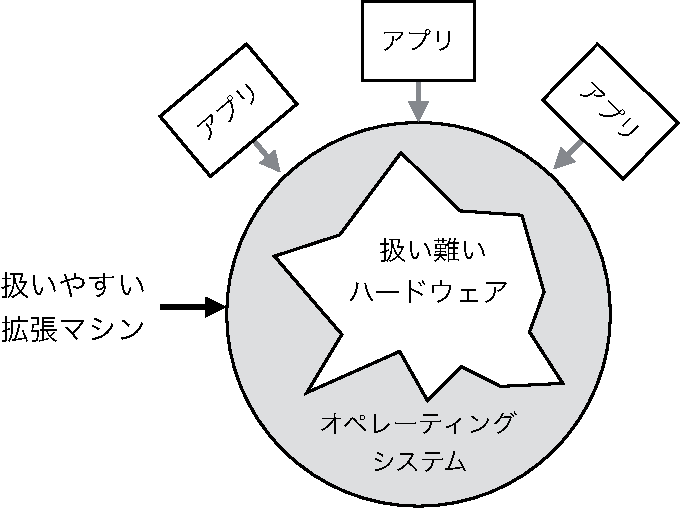
\includegraphics[scale=0.66]{Fig/abstruction-crop.pdf}
\end{myfig}

\subsection{ハードウェア管理プログラムとしてのオペレーティングシステム}
オペレーティングシステムはハードウェア資源を管理・制御し,
アプリケーションプログラムにシステムコール等のサービスを提供する.
\figref{system}はカーネルの役割を説明している.

オペレーティングシステムは,
管理するハードウェア資源をアプリケーションプログラムに割当てる.
複数のアプリケーションプログラムに割り付けるために
資源を\emph{仮想化}して必要な数だけ作り出す.
例えば,CPUは時間を区切って複数のプロセスが共有する
(\emph{時分割多重}による\emph{仮想化}).
メモリはアドレスで区切って複数のプロセスが共有する
(\emph{空間分割多重}による\emph{仮想化}).

\begin{myfig}{btp}{コンピュータシステムの構成}{system}
  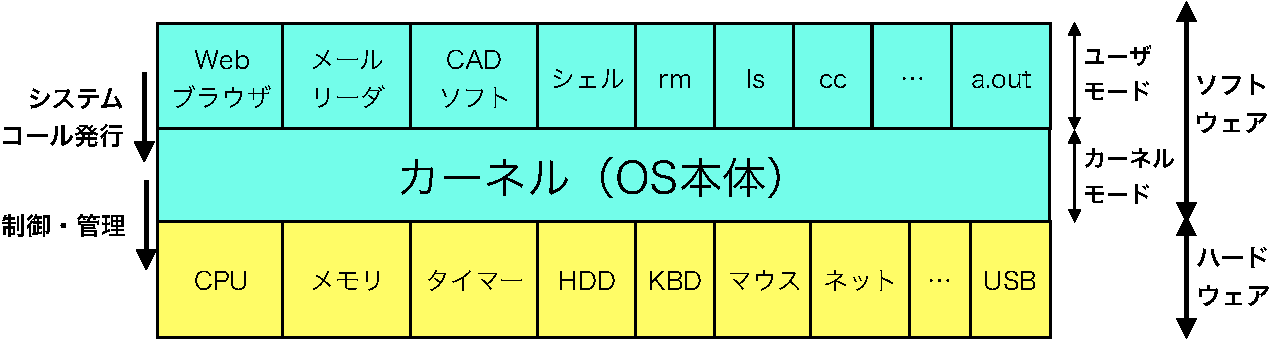
\includegraphics[scale=0.66]{Fig/system-crop.pdf}
\end{myfig}

%==============================================================================
\section{オペレーティングシステムの歴史}

\subsection{第1世代(1945〜1955,真空管の時代)}
初期のコンピュータはコンソールパネルを通して操作する,
巨大なTeC\cite{tec}のようなものだった.
OSは存在せずプログラマはまさにTeCと同様なプログラミングとデバッグを行っていた.

しかし,当時のコンピュータはTeCと異なり大変高価な装置であった.
その高価なコンピュータを一人のプログラマが長時間にわたって
独占使用することになる.
プログラマがバグの原因を考えている間,
とても高価なコンピュータが遊んでしまい勿体ないものであった.

\subsection{第2世代(1955〜1965,トランジスタの時代)}
\label{gen2nd}
コンピュータがトランジスタ回路で製作されるようになり,
\emph{メインフレーム}と呼ばれる大型コンピュータが,
大企業,政府機関や大学等で実用的に使用されるようになった.
メインフレームは数百万ドルと高価だったので,
ハードウェアを遊ばせること無く使用することが優先課題であった.
そこで人手を介すること無く自動的に次々と連続して処理を行う
「コンピュータの自動運転」が行われるようになった.
この処理方式のことは\emph{バッチ処理}と呼ばれた.
\figref{batch}にバッチ処理の概要を示す.

プログラマは\figref{punchcard}のような紙カードに
プログラムやデータを一行ずつ打込む.
100行のプログラムは100枚の紙カードを使用して記録する.
このようにして出来た紙カードの束が一つの処理単位(\emph{ジョブ})になる.
コンピュータでは\emph{バッチモニタ}と呼ばれる常駐プログラムが実行される.
バッチモニタは紙カードからジョブを読み込み実行させる.
ジョブが終了するとバッチモニタに制御が戻り次のジョブが自動的に実行される.
バッチモニタが発展してやがてOSになる.

\begin{myfig}{btp}{バッチ処理}{batch}
  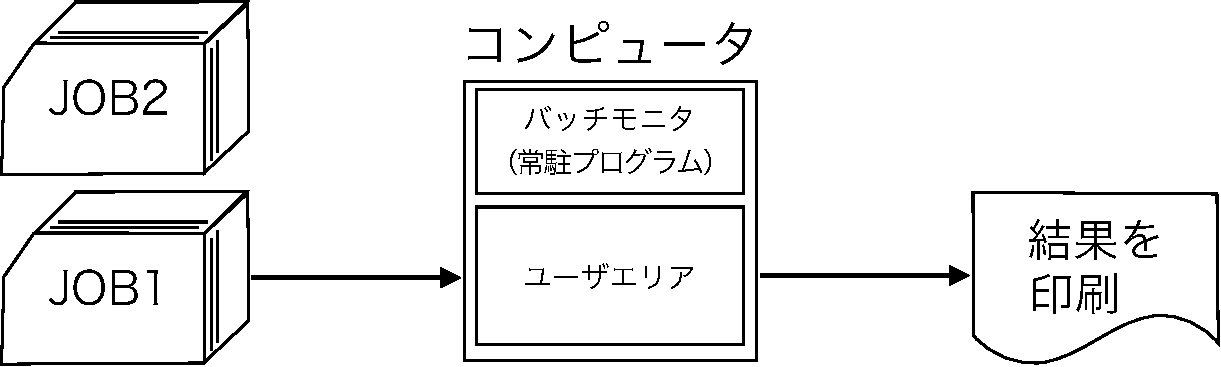
\includegraphics[scale=0.5]{Fig/batch-crop.pdf}
\end{myfig}

\begin{myfig}{btp}{紙カード}{punchcard}
  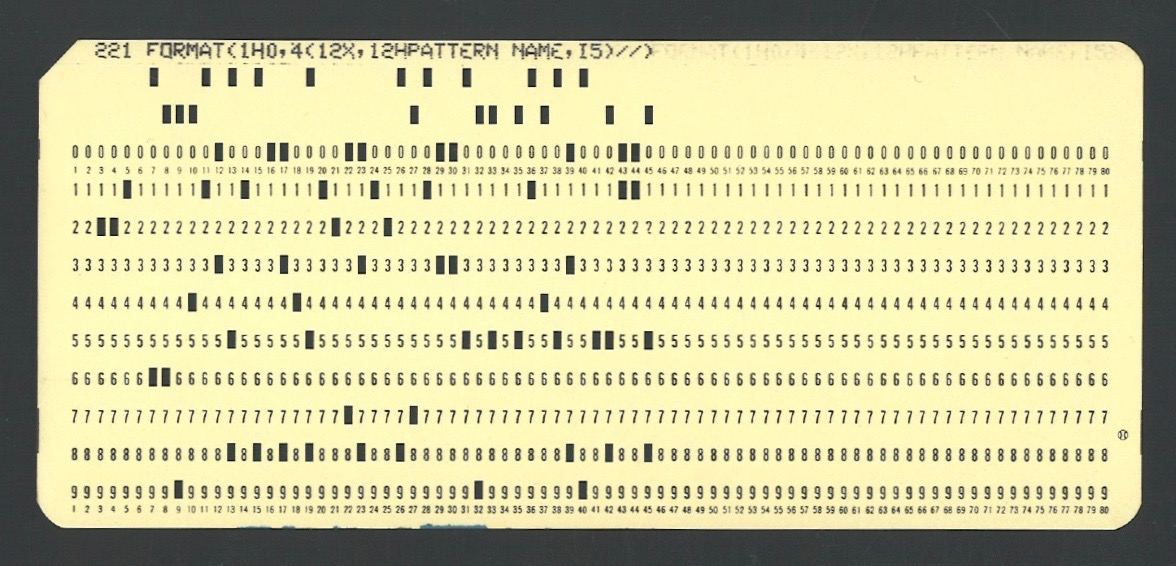
\includegraphics[scale=0.3]{Photo/punchcard.jpg}
\end{myfig}

この方式でうまく処理できるように,次のような発明があった.

\begin{enumerate}
\item \emph{JOB制御言語(JCL : Job Control Language)} \\
  バッチモニタを制御するコマンド言語をJOB制御言語(JCL)と呼ぶ.
  JCLコマンドはジョブ途中の紙カードに記載する.
  \figref{job}にJCLを含むジョブの構成を示す.
  これは,
  FORTRAN言語で記述したプログラムを実行し,
  後半にあるデータを処理するジョブの例になっている.

  \begin{myfig}{btp}{ジョブの構成}{job}
    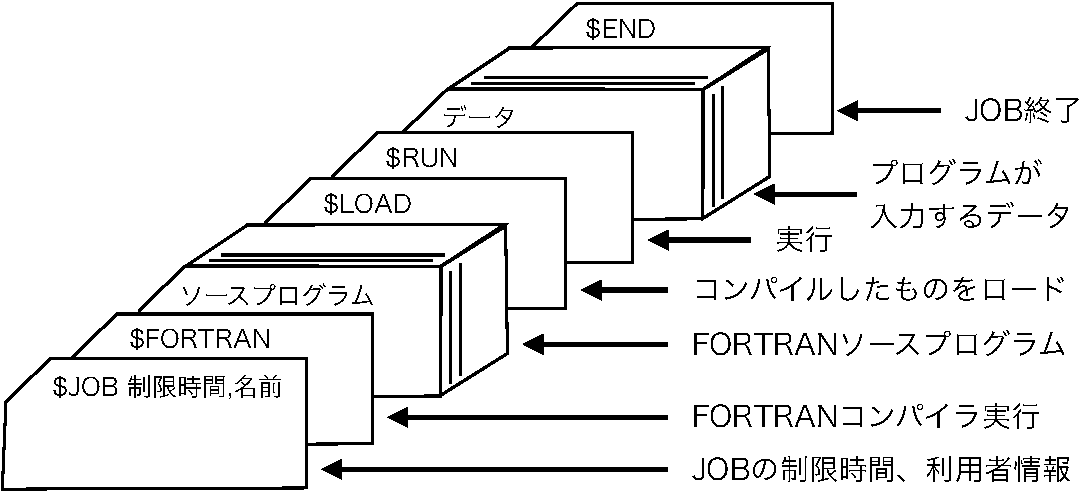
\includegraphics[scale=0.5]{Fig/job-crop.pdf}
  \end{myfig}

\item \emph{実行モード} \\
  ユーザプログラム(ジョブ)のバグで
  バッチモニタが破壊されないようにするために,
  ユーザプログラム実行中なのかバッチモニタ実行中なのか区別する必要がある.
  どちらを実行中なのかを示すハードウェアのフラグを導入し,
  \emph{ユーザモード}と
  \emph{カールモード}(\emph{スーパバイザモード}とも呼ぶ)を
  区別するようになった.
  ユーザモードではハードウェアへのアクセスや,
  実行できる機械語命令に制限がある.

\item \emph{システムコール} \\
  ユーザプログラムが直接に入出力装置等にアクセスすることは,
  バッチ処理を継続できなくする恐れがあるので許されない.
  例えばユーザプログラムがハードウェアのモードを切り換えてしまうと,
  以降のジョブが正常に実行されなくなる恐れがある.
  そこで,ユーザプログラムはバッチモニタに依頼(システムコール)して
  入出力を行う必要がある.

  プログラムが終了する時は
  カーネルモードに切り換えてバッチモニタに戻る必要がある.
  カーネルモードに切り替える機械語命令をユーザプログラムが実行可能だと,
  実行モードが無意味になるので許可すべきではない.
  システムコールを使用してプログラムを終了する.

\item \emph{記憶保護} \\
  ユーザプログラムのバグでバッチモニタが破壊されないように,
  ユーザモードで実行中は
  主記憶のバッチモニタ領域に書込みができないようにする.
\end{enumerate}

\subsection{第3世代(1966〜1980,ICとマルチプログラミングの時代)}
1960年代のコンピュータはIC(Integrated Circuit)を用いて作られるようになり
価格性能比が随分改善された.
第3世代と呼ばれる当時のオペレーティングシステムの中には,
現代のオペレーティングシステムの先祖であったり,
強い影響を与えたものがある.
\figref{tree}に第3世代から現代に至るまでの系統図を示す.


IBMが開発したSystem/360(\figref{system360})は高価な大型のものから,
安価な小型のものまでで同じオペレーティングシステムが使用でき,
同じユーザプログラムを実行できる\emph{シリーズ化}を行い商業的に大成功をおさめた
\cite{third}.
System/360はそれ以前のものとは異なり科学技術計算にも事務処理にも使用できる.
System/360のオペレーティングシステムは,
1966年にデビューしたOS/360である.
\figref{tree}に示すように,
OS/360の子孫であるz/OSが現代でも使用されている\cite{os360}.

\begin{myfig}{btp}{フォルクスワーゲンで使われているSystem/360}{system360}
  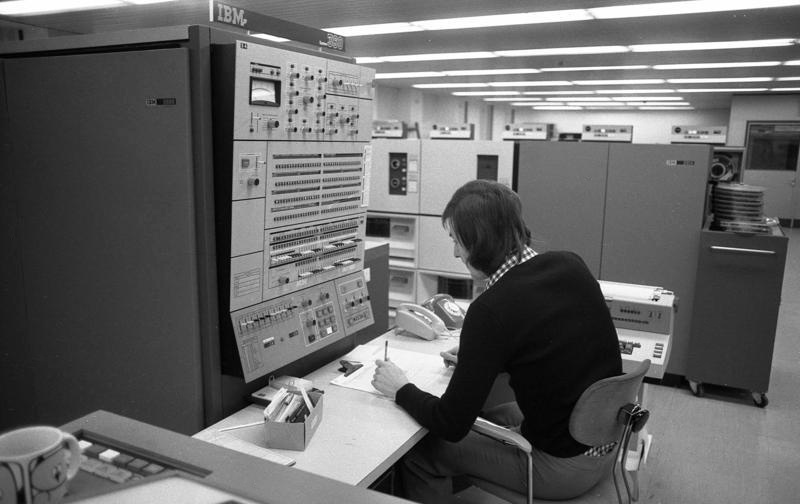
\includegraphics[scale=0.25]
  {Photo/Bundesarchiv_B_145_Bild-F038812-0014,_Wolfsburg,_VW_Autowerk.jpg}\\
  {\small
    ウィキメディア /
    Bundesarchiv, B 145 Bild-F038812-0014 /
    Schaack, Lothar / CC-BY-SA 3.0 de}
\end{myfig}

OS/360を含む第3世代のオペレーティングシステムが
実現した重要な新しい機能を紹介する.

\begin{itemize}
\item \emph{仮想記憶} \\
  主記憶を仮想化し実際より大きい主記憶があるように見せる.
  実際の主記憶より大きいプログラムが実行可能になる.

\item \emph{マルチプログラミング} \\
  \label{multiprogramming}
  \figref{multiprogramming}のように,
  複数のプログラム(ジョブ)を主記憶にロードしておき,
  その中で実行可能なものを選んで実行する.
  入出力待ち等で実行できなくなったら他のプログラムを実行する.
  高価なCPUが入出力待ちで停止する可能性を低くすることができた.

  \begin{myfig}{btp}{マルチプログラミングシステム}{multiprogramming}
    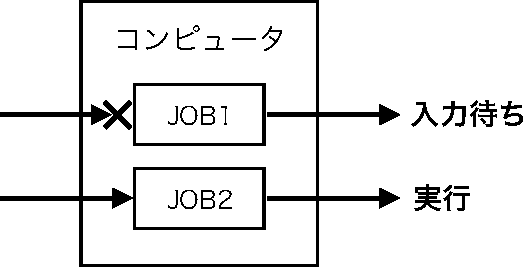
\includegraphics[scale=0.66]{Fig/multiprogramming-crop.pdf}
  \end{myfig}

\item \emph{タイムシェアリング(TSS:Time Sharing System)} \\
  マルチプログラミングの一種である.
  \figref{timesharing}のように,
  複数のターミナルをコンピュータに接続し
  複数のユーザが同時にコンピュータを使用できるようにする.
  短時間(例えば10ms)で処理するジョブを次々に切り換えることで,
  ユーザは自分がコンピュータを独占しているように感じることができる.
  なお,ターミナルは\figref{terminal}のような,
  キーボードと表示装置だけを備えた安価な装置である.

  \begin{myfig}{btp}{タイムシェアリングシステム}{timesharing}
    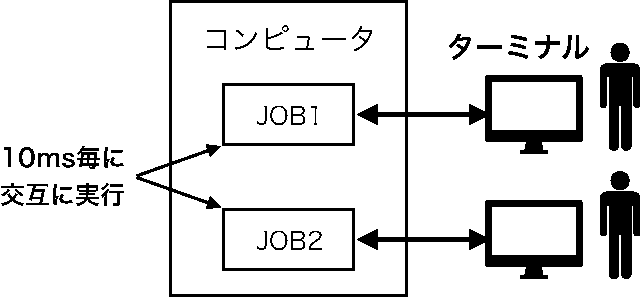
\includegraphics[scale=0.66]{Fig/timesharing-crop.pdf}
  \end{myfig}

  \begin{myfig}{btp}{ターミナル}{terminal}
    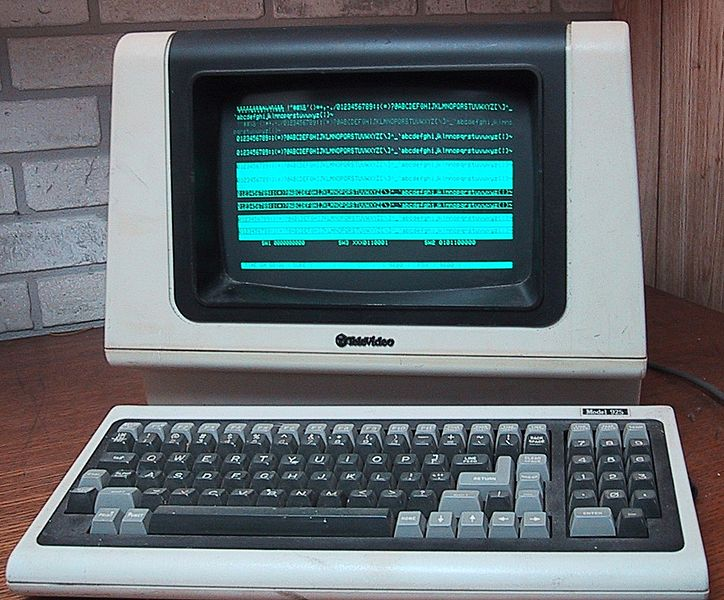
\includegraphics[scale=0.25]
     {Photo/724px-Televideo925Terminal.jpeg}\\
     {\small 写真:
       \url{http://commons.wikimedia.org/wiki/File:Televideo925Terminal.jpg}
       (パブリックドメイン)}
  \end{myfig}
\end{itemize}

この時代のオペレーティングシステムやコンピュータシステム,
そして,それらの開発プロジェクトの中で,
その後のオペレーティングシステムに多くの影響を与えた有名なものを紹介する.

\begin{itemize}
\item OS/360 \\
  世界初の本格的な商用オペレーティングシステムである.
  メインフレームの主流OSとなり子孫は現在でも使用されている\cite{os360}.

\item MULTICS(MULTiplexed Information and Computing Service)プロジェクト
  \cite{third} \\
  MIT,ベル研究所,General Electricが共同で始めた
  巨大で強力なコンピュータシステムを構築するプロジェクトである.
  強力な一台のコンピュータで
  都市一つ分のコンピュータサービスを提供する構想だった.
  完成までに長い期間を要し(その間にベルとGEが脱落し),
  商業的には失敗であったがその後のオペレーティングシステムに影響を与える
  多くのアイデアが出てきた.

\item UNIX(ユニックス) \\
  MULTICSプロジェクトから抜けたベル研のKen Thompsonらにより開発された
  \cite{unix}.
  \figref{tree}に示すように,
  現代のオペレーティングシステムの多くがUNIXを起源にしている.
  子孫ではないものもUNIXの影響を強く受けている.
  LinuxはUNIX互換のオペレーティングシステムを作ろうとして
  開発が始まった\cite{linux}.
  Androidの中身はLinuxである\cite{android}.
  z/OSはUNIX互換環境を備えている\cite{zos}.
  WindowsにもUNIX互換環境(POSIXサブシステム)を
  利用可能なものがある\cite{windows}.

\item DynaBook(ダイナブック:OSだけでなくコンピュータ全体を指す)
  \cite{dynabook2} \\
  アラン・ケイが1972年に著した
  「A Personal Computer for Children of All Ages」\cite{key72, key72J}
  に登場する理想のパーソナルコンピュータである.
  アラン・ケイがゼロックスのパロアルト研究所に在籍中の1970年代に開発した
  Alto上の「暫定ダイナブック環境」(\figref{smalltalk})は
  既にGUIやマウスを使用していた.
  スティーブ・ジョブスがAltoを見たことが
  LISA開発きっかけになったと言われている\cite{dynabook}.

  \begin{myfig}{btp}
    {Alto(Alto エミュレータ)のスクリーンショット}
    {smalltalk}
    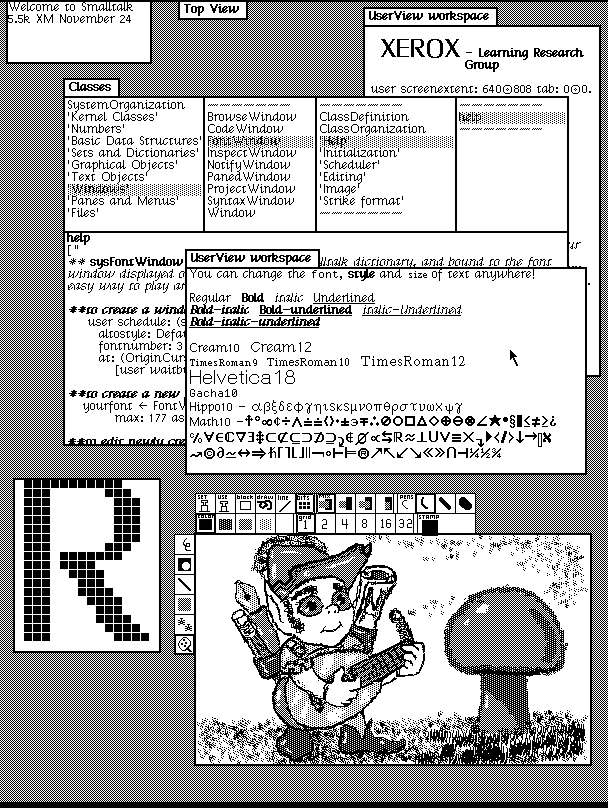
\includegraphics[scale=0.5]{Photo/Smalltalk-76.png}\\
                    {\small
                      ウィキメディア /
                      SUMIM.ST /\\
                      AltoやNoteTakerで動作した
                      アラン・ケイ達の暫定Dynabook環境
                      (Smalltalk-76、同-78の頃) /
                      CC-BY-SA 4.0
                    }
  \end{myfig}

\end{itemize}

\subsection{第4世代(1980〜現代,PCの時代)}

1970年代に単一のLSIにCPU全体を集積したマイクロプロセッサが登場した.
1970年代中頃にはマイクロプロセッサを用いて個人向けのコンピュータである
パーソナルコンピュータ(当時はマイクロコンピュータと呼んでいた)
を作ることが可能になった.
それに伴いパーソナルコンピュータ用のオペレーティングシステムが登場した.

\begin{enumerate}
\item 8bitマイクロコンピュータの時代 \\
  1977年にDigtal Reserch社がCP/M(Control Program for Microcomputer)と呼ばれる
    8bitマイクロコンピュータ用の簡単なオペレーティングシステムを
    開発し成功した.
    しかしこのオペレーティングは16bitパーソナルコンピュータの時代には
    早々に消え去ってしまった\cite{fourth}.

  \item 16bitパーソナルコンピュータの時代 \\
    IBMが1981年に16bitパーソナルコンピュータIBM PC\cite{ibmpc81}
    (\figref{ibmpc})を発売した.
    IBM PCは現在のWindows PCの先祖である.
    IBM PCの子孫は改良や拡張を続けながら現在まで高いシェアを維持し続けている.
    IBM PCのオペレーティングシステムとして開発されたのが,
    Microsoft社のMS-DOS(MicroSoft Disk Operating System)\cite{msdos}である.
    バージョン2からはUNIXのような
    階層ディレクトリやパイプ,リダイレクト等の機能を持っている.
    \figref{tree}に示すように,MS-DOSはWindowsに置き換わりWindows MEまで
    バージョンアップが繰り返された.

    \begin{myfig}{btp}{IBM PC}{ibmpc}
      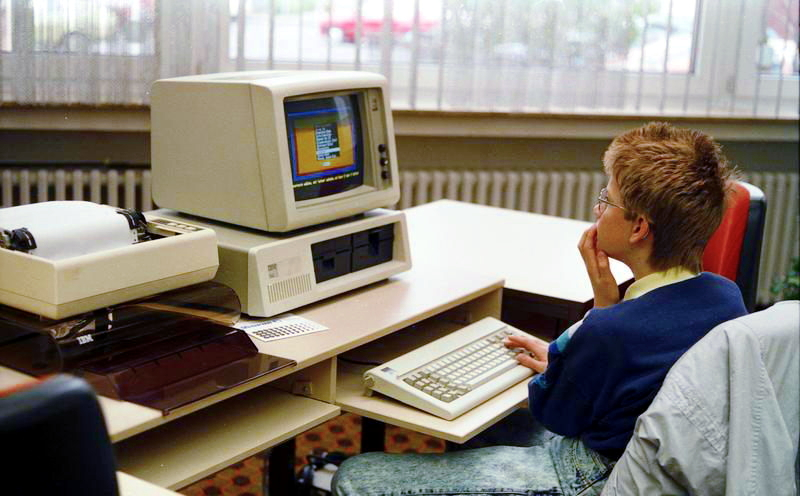
\includegraphics[scale=0.35]
                      {Photo/Bundesarchiv_B_145_Bild-F077948-0006,_Jugend-Computerschule_mit_IBM-PC.jpg}\\
                      {\small
                        ウィキメディア /
                        Bundesarchiv, B 145 Bild-F077948-0006 /
                        Engelbert Reineke / CC-BY-SA 3.0 de}
    \end{myfig}

    Apple社は1984年にMacintosh(\figref{macintosh})を発売した.
    MachintoshのOSであるMacOSはLISAを経てDynaBook\cite{key72, key72J}の
    影響を受けていると言われている\cite{fourth}.
    \figref{tree}に示すように,
    当初のMacOSはMacOS 9\cite{classicmacos}まで改良が続けられた.

    \begin{myfig}{btp}{初代Macintosh}{macintosh}
      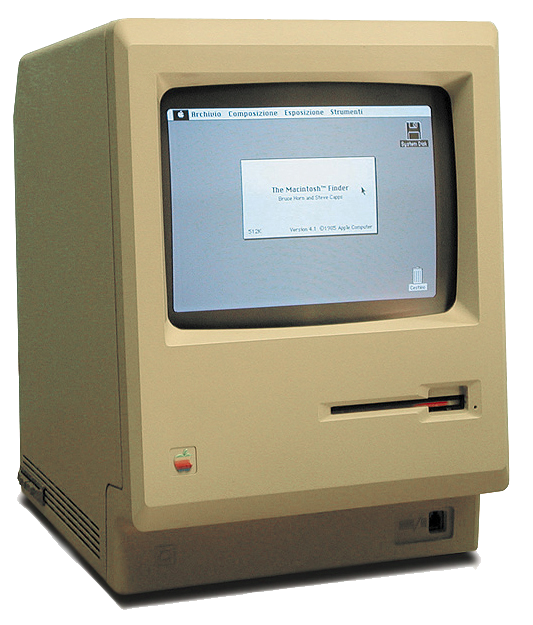
\includegraphics[scale=0.25]{Photo/Macintosh_128k_transparency.png}\\
                      {\small
                        ウィキメディア / w:User:Grm wnr /
                        File:Macintosh 128k transparency.png /GFDL}
    \end{myfig}

  \item 32bitパーソナルコンピュータの時代 \\
    1990年頃には32bitのマイクロプロセッサが
    パーソナルコンピュータにも使用されるようになった.
    32bitのマイクロプロセッサは実行モードを備え,
    またメモリ管理ユニットも利用可能であった.
    つまり,カーネルモードとユーザモードを使い分けたり
    仮想記憶を利用する本格的な第3世代のオペレーティングシステムを
    実行できる環境がパーソナルコンピュータにも整った.

    そこで,
    従来ワークステーションやミニコンで使用されていた
    UNIXを安価なパーソナルコンピュータ(特にIBM PC互換機)で
    動くようにする人たちが現れ,
    オープンソースソフトウェアとしてLinuxやFreeBSD等の開発が始まった.
    また,もともとパーソナルコンピュータ用のWindowsやMacOSも
    32bitマイクロプロセッサの機能を使いこなす
    本格的なオペレーティングシステムに生まれ変わった.

    \begin{itemize}
    \item Linux \\
      1991年に開発が始まったLinuxはUNIX互換のオペレーティングシステムを
      パーソナルコンピュータ(IBM PC互換機)用に
      独自に作成したものである\cite{linux}.
      Linuxは改良され続け,
      現在ではパーソナルコンピュータだけでなく,
      スーパーコンピュータ「京」のオペレーティングシステム\cite{kei}から,
      スマートフォンのオペレーティングシステムであるAndroid\cite{android},
      テレビ等の組込みシステムのオペレーティングシステムまで,
      広く使われるようになっている.

    \item BSD 系の UNIX \\
      386BSD\cite{386bsd}はBSD UNIXをIntel 80386 CPUを搭載した
      パーソナルコンピュータ(IBM PC互換機)で動作するようにしたものである.
      386BSDはFreeBSD等に受継がれるがUNIXのライセンス問題が発生する\cite{unix}.
      ライセンス問題が片付き安心して使用できるようになった
      4.4BSD-Lite Release 2\cite{unix}をベースに
      FreeBSD, NetBSD, OpenBSD 等の多くの BSD 系 PC-UNIXが開発された.

      その後,FreeBSDは MacOS X に取り込まれている.
      また,FreeBSDにZFSが移植された\cite{zfs}ので
      ファイルサーバ用に特化したFreeNAS\cite{freenas}にも使用されている.
      なお,徳山工業高等専門学校・情報電子工学科のパソコン室では
      1993年10月に386BSDの利用を開始して以来,
      2014年3月までFreeBSDを学生用PCやサーバのオペレーティングシステムとして
      使用してきた\cite{iebsd}.

    \item System V 系の UNIX \\
      System V の流れを汲むSolaris\cite{solaris}は,
      RISC マイクロプロセッサ SPARC を搭載するサーバやワークステーションでも,
      パーソナルコンピュータ(IBM PC 互換)でも使用できる.

    \item 従来のパーソナルコンピュータ用オペレーティングシステム \\
      従来のWindowsやMacOSはCPUの実行モード等を使用していなかったので,
      アプリケーションプログラムのバグにより
      システム全体が停止するようなトラブルを防ぐことができなかった.
      そこで,32bitマイクロプロセッサの使用を前提に新しく作り直された.

      新しく作り直された32bitのWindows NT系列の製品は,
      徐々に従来のWindowsを置換えた.
      (\figref{tree}参照).
      現在(2017年10月)の最新版はWindows 10である.

      MacOS は,2001年にUNIXの流れを汲み安定して動作するOPENSTEPベースの
      MacOS X\cite{macos}に置き換わった(\figref{tree}参照).
      その後,名称が OS X, macOS と変更されたがこれらは MacOS X の改良版である.
      現在(2017年10月)の最新版はmacOS 10.13 High Sierraである.
      iPhoneのiOSはMacOS Xをタッチパネル用に再構成したものである\cite{ios}.
    \end{itemize}
\end{enumerate}

\subsection{インターネット世代}
現在のオペレーティングシステムはTCP/IP機構が組込まれ
インターネットに接続することができる.
今ではパーソナルコンピュータやスマートフォンの使用を
インターネット抜きに考えることができない.
オペレーティングシステムにとってインターネットに接続できることは
重要なことである.

TCP/IPを実装した4.2BSDが1984年に公開された\cite{bsd}.
以来,4.2BSDの子孫はインターネットに対応している.
1988年に公開されたSystem V R4はBSD起原のTCP/IPの実装を含んでいた\cite{svr4}.
これの子孫もインターネットに対応している.
Linuxも1.0の頃にはTCP/IPの実装を含んでいた\cite{linux1}.
WindowsはWindows 95からTCP/IPを標準装備している\cite{windows}.
MacOSはMacOS 8が発表されるまでにはインターネット対応がされていた
\cite{classicmacos}.
メインフレームの世界でもOS/390はインターネットに対応した\cite{os390}.

このようにして1990年代の後半には多くのオペレーティングシステムが
インターネット対応を完了させた.
インターネット対応を完了させたオペレーティングシステムを
「インターネット世代のオペレーティングシステム」と言うことができる.

\begin{myfig}{btp}{オペレーティングシステムの系統図}{tree}
  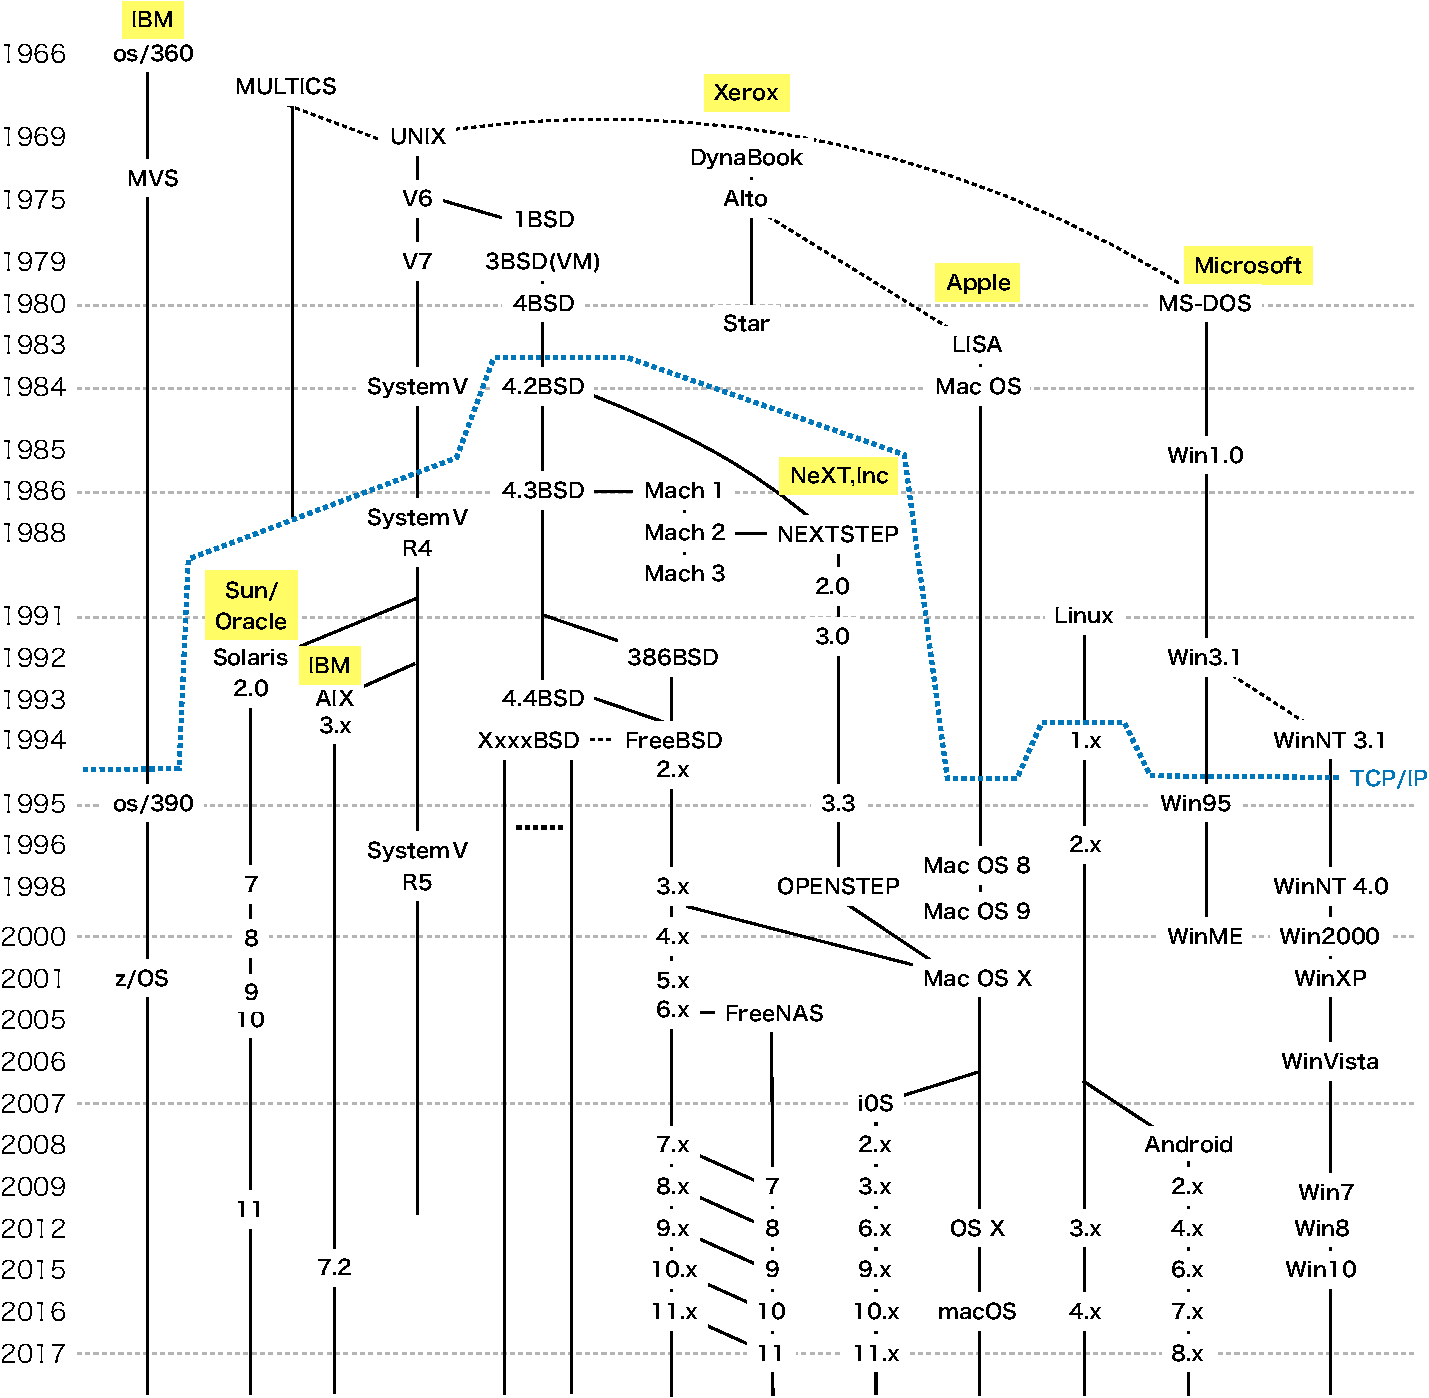
\includegraphics[scale=0.6]{Fig/tree-crop.pdf}\\
                  {\small
                    系統図は\cite{os360,
                      mvs,
                      os390,
                      zos,
                      unix,
                      solaris,
                      aix,
                      mach,
                      bsd,
                      bsdd,
                      386bsd,
                      freebsd,
                      freenas,
                      nextstep,
                      classicmacos,
                      dynabook,
                      macos,
                      ios,
                      linux,
                      android,
                      msdos,
                      windows}
                    の内容を総合して作成した.}
\end{myfig}

%==============================================================================
\section{まとめ}
狭義のオペレーティングシステムは\emph{カーネル}のことを指す.
本書は狭義のオペレーティングシステムについて述べている.

オペレーティングシステムの重要な役割りは,
コンピュータの資源を\emph{抽象化}することと\emph{仮想化}することである.
オペレーティングのユーザは,
使いやすい抽象化されたインタフェースを通して資源を利用できる.
また,ユーサは仮想化された資源を必要なだけ独占して使用することができる.

オペレーティングシステムは,
1950年代に出現したバッチモニタから進化してきた.
現在では,
スーパーコンピュータから組み込み用コンピュータまで,
非常に広い範囲のコンピュータが本格的なオペレーティングシステムを搭載している.


%==============================================================================
\section*{練習問題}
\begin{enumerate}
  \renewcommand{\labelenumi}{\ttfamily\arabic{chapter}.\arabic{enumi}}
  \setlength{\leftskip}{1em}
\item \emph{抽象化}について説明しなさい.
\item \emph{抽象化}の例をいくつか挙げなさい.
\item \emph{仮想化}について説明しなさい.
\item \emph{仮想化}の例をいくつか挙げなさい.
\item 自分がいつも使用しているコンピュータやスマートフォンの
  オペレーティングシステムの種類を調べなさい.
\end{enumerate}
 % オペレーティングシステムとは
\chapter{前提知識}
以下では,
本書で想定しているコンピュータのハードウェアやソフトウェアの
構成について解説する.

\section{コンピュータのハードウェア構成}
本書は,
コンピュータのハードウェア構成が\figref{hardBlock}のようになっている
ことを前提にしている.
複数のCPU(Central Processing Unit)がメモリを共有し,
また,全てのCPUは同じ機能を持ち優劣が無い.
このような方式を
{\bf SMP(対称型マルチプロセッシング:Symmetric Multiprocessing)}と呼ぶ.
メモリはCPUだけでなく,
I/Oコントローラ(\figref{hardBlock}ではアダプタやコントローラ)にも
共有される.

\myfigure{btp}{scale=0.48}{Fig/hardBlock-crop.pdf}{ハードウエア構成}{hardBlock}

\begin{enumerate}
\item CPU \\
CPUはコンピュータの頭脳である.
図はCPUが二つの構成になっているが,
実際は一つの場合も,もっと多い場合もある.

\item メモリ(主記憶装置) \\
プログラムやデータを記憶し,
プログラム実行する際にCPUが直接使用する記憶装置である.

\item タイマー \\
一定間隔で繰り返しCPUに割り込みを発生するインターバルタイマーである.

\item グラフィックアダプタ \\
ディスプレイを接続するためのアダプタである.
表示内容を記憶するメモリを独自に持つ場合と,
主記憶装置を使用する場合がある.
最近のパーソナルコンピュータでは,
グラフィックアダプタにGPU(Graphics Processing Unit)が組込まれている.

\item SATA ホストコントローラ \\
SATA(Serial Advanced Technology Attachment)は,
パーソナルコンピュータと二次記憶装置(ハードディスクやCD-ROM)を接続するための
インタフェース規格である.
SATA ホストコントローラは次のような動作をする.
\begin{enumerate}
\item CPUがSATAホストコントローラにコマンドを書き込む.
コマンドは,
「読み/書き」,「セクタアドレス」,「セクタ数」,「メモリアドレス」
を含んだものである.
\item SATAホストコントローラは,
ディスクコントローラと通信しハードディスクにコマンドを渡す.
\item ハードディスクの読み・書きが可能になったら,
ホストコントローラはハードディスクとメモリの間でデータ転送を行う.
このようなCPUを介さないデータ転送のことを,
{\bf DMA(Direct Memory Access)}と呼ぶ.
\item SATAホストコントローラはCPUに割り込み信号を送り,
データの転送が完了したことを知らせる.({\bf I/O完了割り込み})
\end{enumerate}
CPUは,
SATAホストコントローラにコマンドを送ってから割り込みが発生するまでの間,
他の仕事をすることができる.
ハードディスクの操作(I/O操作)とCPUの計算は並列実行される.

\item USBコントローラ \\
USB(Universal Serial Bus)は,
パーソナルコンピュータと周辺装置を手軽に接続できるインタフェースである.
USBメモリスティックやプリンタ,キーボード,マウス等,多くの周辺装置が
USBを通して接続できる.
USBコントローラもSATAホストコントローラのようにDMA機能を備えている.

\item ネットワークアダプタ \\
パーソナルコンピュータのネットワークアダプタは,
GbE(Gigabit Ethernet)規格のものが普及している.
これもSATAホストコントローラのようにDMA機能を備えている.

\item BUS(バス) \\
パーソナルコンピュータのハードウェアを構成する装置の間で
データをやり取りするための配線である.
CPUだけでなくDMAを使用するコントローラやアダプタが大量のデータ転送を行うので,
バスのデータ転送能力がパーソナルコンピュータの性能向上のボトルネックになる.

そのため後で説明するように,実際の物理的な接続は\figref{hardBlock}とは
かなり異なった構成になっている.
しかし,オペレーティングシステムが意識しなければならない論理的な
接続は\figref{hardBlock}のようなものである.

\end{enumerate}

\section{CPUの構成}
本書では、CPUは\figref{cpuBlock}のような部品で構成されると考える.
\figref{hardBlock}に示したように,CPUはBUSを通して他の装置と接続される.
CPUは,一つの機械語命令の実行が終わり次の命令の実行を開始する前に,
他の装置から割り込みを受け付けることができる\footnote{
例外的に,メモリ管理に関する一部の割込は機械語命令の途中で発生する.}.

\myfigure{btp}{scale=0.66}{Fig/cpuBlock-crop.pdf}{CPUの構成}{cpuBlock}

\begin{enumerate}
\item {\bf PSW(Program Status Word)} \\
PSWは,PC(Program Counter)とFlags(フラグ)から構成されるものとする
\footnote{
教科書によっては,フラグだけをPSWと呼ぶ場合もある.}.
PCはCPUが実行中のプログラムの命令アドレスを保持するカウンタである.
Flagsは計算の結果によって変化するフラグの他に,
割り込み許可/不許可を表現するビット,
実行モード(ユーザモード/カーネルモード)を表現するビット等が含まれる.

\item {\bf CPUレジスタ} \\
計算に使用するCPUの汎用レジスタのことである.
TeCではG0,G1,G2,SPのこと,
情報処理技術者試験のCOMETではGR0,GR1,GR2,GR3,GR4のことである.

\end{enumerate}

PSWとCPUレジスタは,
機械語命令を実行する毎に値が変化・確定しプログラムが意識している\footnote{
一方でCPU内部にはプログラムから見えないレジスタもある.
}ので,CPUを仮想化し実行するプロセスを切換える際に保存・復旧の対象となる.

\section{最近のコンピュータの実際の構成}

Intel社のCPUを使用したデスクトップ・パーソナルコンピュータと
サーバコンピュータの構成を説明する.
バスがボトルネックにならないように,
CPUにメモリを直接接続してある.

\subsection{デスクトップ・パーソナルコンピュータ}
\figref{intelDesktop}はIntel社のCPUを使用した
近年のデスクトップ・パーソナルコンピュータの構成を表している.
Intel社の用語では,これまで「CPU」と読んでいたものが
「{\bf Core(コア)}」と呼ばれる.
「CPU」は複数のコアを含んだLSIのことを指している.
デスクトップ用のCPUには1〜4個のコアが集積されている.

コアに隣接しているL1はレベル1キャッシュ(Level 1 cache)を表している.
L2は複数のコアにシェアされるレベル2キャッシュ(Level 2 cache)を表している.
メモリとのデータ転送量が多いCoreとGPUがCPUに集積され,
I/O装置のコントローラやアダプタはPCHに集積されている.
CPUとPCHはDMIと呼ばれる専用のインタフェースを用いて接続される.

\myfigure{btp}{scale=0.66}{Fig/intelDesktop-crop.pdf}
{デスクトップPCの構成}{intelDesktop}

\subsection{サーバコンピュータ}
より強力な処理能力が必要なサーバ用コンピュータでは,
\figref{intelServer}のように多くのコアを内蔵するCPUを複数個使用する.
現在(2017年秋)最新の Intel Xeon Processor Scalable Family の場合,
CPU同士はUPIと呼ばれる高速な専用インタフェースで接続される.
最大の構成は,28コアのCPUを8個使用し合計224コアのものである.
PCHもサーバ用のものでは,より多くのストレージやネットワークを接続できる.

\myfigure{btp}{scale=0.5}{Fig/intelServer-crop.pdf}
{サーバPCの構成}{intelServer}

\section{オペレーティングシステムの構造}
\figref{osOrganization}にオペレーティングシステムの構造を示す.
オペレーティングシステムのカーネルは
\figref{osOrganization}中央部分のソフトウェアである.
ユーザプロセスはユーザモードで,
カーネルはカーネルモードで実行される.

\subsection{カーネルの構成}
\figref{osOrganization}に示すように,
カーネルは以下のようなモジュールから構成される.

\begin{enumerate}
\item {\bf 割り込みハンドラ} \\
割込みが発生した時に自動的に実行される割込み処理ルーチンである.
割込みが発生した原因を判断し,必要なモジュールを呼出す.
例えば,タイマーからの割込みならタイマーのデバイスドライバを呼出す.

\item {\bf ディスパッチャ} \\
カーネルの処理が終了した時,
実行可能なプロセスの中から一つを選んで実行を再開させる.

\item {\bf コア} \\
割込みハンドラとディスパッチャを含むコアは,
資源の仮想化を行うために必ずカーネルモードで実行される必要がある部分である.

\item {\bf サービスモジュール} \\
サービスモジュールは,
ハードウェアを抽象化した便利なコンピュータを
ユーザ・プロセスに提供するためのプログラムである.
\end{enumerate}

\myfigure{btp}{scale=0.66}{Fig/osOrganization-crop.pdf}
{オペレーティングシステムの構造}{osOrganization}

\subsection{カーネルの動作概要}
通常,コンピュータはユーザ・プロセスを実行し目的の仕事をしている.
何かイベントが発生すると割込みによりCPUに通知される.
CPUはカーネルモードに切り替わり割込みハンドラに制御を移す.
CPUがユーザ・プロセスの実行からカーネルの実行に移行するのは,
{\bf 割込みが発生した時だけ}である.

\subsubsection{割込み原因}
\label{interruptSource}
カーネルへ実行を移すには割込みを発生する以外に方法がない.
割込みが発生する原因には以下のようなものがある.
システムコール以外はユーザ・プロセスが意図しない間に発生する.

\begin{enumerate}
\item I/O完了・タイマー \\
ホストコントローラやネットワークアダプタ,タイマーのようなハードウェアが,
コマンドの実行完了等をCPUに知らせるために発生する.

\item システムコール \\
ユーザ・プロセスは,
割込みを発生する特殊な機械語命令である{\bf SVC(Supervisor Call)}命令
\footnote{
CPUによってはTRAP命令,INT命令と呼ばれることもある.
}
を用いて
システムコールを発行する.
カーネルはSVC命令実行時のCPUレジスタの値などから
システムコールの種類やパラメータを知ることができる.

\item 保護違反 \\
ユーザ・プロセスが,
ユーザ・モードでは実行が許可されない命令を実行したり,
アクセスが許可されないメモリ領域をアクセスした場合に発生する.

\item ソフトウェアのエラー \\
ユーザ・プロセス実行中に計算でオーバーフローが発生したような時に発生する.

\item ハードウェアのエラー \\
ハードウェアの故障や電源の異常を検知した時に発生する.

\end{enumerate}

\subsubsection{割込み発生時のカーネルの動作}
割込みが発生するとカーネル・モードに切り換わり割込みハンドラに制御が移る.
その後,カーネル内では以下のような手順で処理がされる.

\begin{enumerate}
\item 割込みハンドラは後でプロセスの実行を再開できるように,
プロセスのCPUの状態({\bf コンテキスト}:PSW,CPUレジスタ)を保存する.

\item 割込みハンドラは割込み原因を調べ,
原因に応じたカーネル内のサービスモジュールやデバイスドライバに制御を渡す.
例えばファイル操作のシステムコールならファイルシステムへ制御を渡す.

\item サービスモジュールやデバイスドライバの処理が終了したら
ディスパッチャに制御が渡される.
ディスパッチャは実行可能なプロセスの一つを選び,
コンテキストを復旧しプロセスの実行を再開させる.
\end{enumerate}

\subsection{プロセスの構造}
\figref{osOrganization}のユーザ・プロセス部分を詳しく描いたものを
\figref{procOrganization}に示す.
プロセスを構成する各部を以下で説明する.

\myfigure{btp}{scale=0.66}{Fig/procOrganization-crop.pdf}
{プロセスの構造}{procOrganization}

\begin{enumerate}
\item {\bf 仮想CPU} \\
CPUを仮想化し,
プロセス毎にCPUが存在するように見せることで,
マルチプログラミングを可能にする.
プロセスがCPUを使用する時間を区切り,
次々に切替える時分割多重によりCPUの仮想化は達成される.

他のプロセスがCPUを使用している間に,
プロセスのコンテキストを保存する領域を仮想CPUと呼ぶことにする.
ハードウェアの実CPUに対応してPSWとCPUレジスタの保存先が必要である.
前の節で説明したように,
プロセスからカーネルに制御が移る時にプロセスのコンテキストを保存する.
プロセス実行時にはコンテキストが実CPUにロードされる.

\item {\bf 仮想メモリ空間} \\
メモリを仮想化しプロセス毎に専用のメモリ空間が存在するように見せかける.
実現方法は第?章の「メモリ管理」で詳しく学ぶ.
仮想メモリ空間は次の部分から構成される.

\begin{enumerate}
\item プログラム \\
機械語プログラムがここに配置される.
C言語で記述されたプログラムの場合,
関数の実行文(式文,if文,for文,while文など)が
翻訳された機械語が該当する.

\item データ \\
プログラムの変数部分がここに配置される.
C言語ではグローバル変数が該当する.

\item ヒープ \\
プログラム実行時に動的に拡大される領域である.
C言語の\|malloc()|関数はヒープに新しい領域を確保する.
\|malloc()|関数が使用される度にヒープ領域は後ろに向かって拡大していく.

\item スタック \\
プログラム実行時にメモリ空間の最後から前に向かって伸びて行く領域である.
サブルーチン・コール時に戻りアドレスを保存したり,
C言語のローカル変数や関数引数を置いたりするために使用される.

\end{enumerate}

\item {\bf プロセス情報} \\
名前にあたる「プロセス番号」,
実行中/実行可能/待ちのどの状態なのか表す「プロセスの状態」,
使用しているメモリの大きさ等を表す「メモリ管理情報」,
CPUを使用した時間を表す「CPU時間」等の情報のことである\footnote{
これらはUNIXのpsコマンドで表示することができる.}.
その他に,プロセスが現在オープンしているファイルに関する情報や,
親プロセス,子プロセス,シグナルハンドラの登録状況,
プロセスの優先度など,様々な情報がここに記録される.
\end{enumerate}

\section{カーネルの構成方式}
カーネルが動作不良を起こすと
実行中の全てのユーザ・プロセスを巻き込んでシステムが停止するので,
カーネルには非常に高い信頼性が要求される.
しかし,カーネルは非常に大きなプログラムになりがちであり\footnote{
Linux や Windows のカーネルのソースコードは500万行にもなる\cite{lines}.},
高い信頼性を確保するにはカーネルの構成方法に工夫が必要である.
%一方でカーネルの処理が重くなると全てのユーザ・プロセスに影響するので,
%効率も犠牲にすることはできない.

\subsection{単層カーネル(モノリシック・カーネル)}
最も一般的な構成方法である.
\figref{osOrganization}のカーネルは単層カーネルの例になっている.
カーネル内の全てのモジュールがリンクされ,一つのプログラムになる.
カーネル内でモジュールの呼出しはCALL機械語命令を用いて行うので効率が良い.
しかし,モジュール同士が密にリンクされているので,
モジュール間で情報の隠蔽がし難くバグが入りやすい.
また,全てのモジュールがカーネル・モードで実行されるので,
一つのモジュールのバグが致命的な結果を引き起こす.
LinuxやFreeBSDは,この方式のカーネルを持つ.

\subsection{マイクロカーネル(micro-kernel)}
\figref{osOrganization}の「コア」からデバイスドライバを取り除き\footnote{
タイマーのデバイスドライバはCPUの仮想化に必要なので,マイクロカーネルに残す.},
カーネル(マイクロカーネル)とし構成する方式である.
\figref{microkernel}にマイクロカーネル方式の概要を示す.
カーネル・モードで実行されるのはマイクロカーネルだけである.

\myfigure{btp}{scale=0.66}{Fig/microkernel-crop.pdf}
{マイクロカーネル方式}{microkernel}

サービスモジュールはカーネルから独立したサーバ・プロセスとし,
権限の低いユーザ・モードで実行される.
ユーザ・プロセスは,マイクロカーネルが提供する
{\bf IPC(プロセス間通信:Inter-Process Communication)}を用いて,
サーバ・プロセスにサービスを要求する.
サーバ・プロセス同士,サーバ・プロセスとデバイスドライバ・プロセスも
IPCを用いて通信する.

デバイスドライバはI/Oポートにアクセスするのでカーネル・モードで
実行される必要があると考えられるが,
I/Oポートへのアクセスをマイクロカーネルのシステムコールに置換えることで,
デバイスドライバもユーザ・プロセスとして実装することが可能である.
この場合は,デバイスドライバがアクセスしても良いI/Oアドレスの範囲内かどうか,
マイクロカーネルがチェックすることが可能である.

マイクロカーネル方式は,
サービスモジュールやデバイスドライバが権限の低いプロセスとして実行されるので,
これらのバグでシステム全体が停止する危険性が低い。
また,
サービスモジュールやデバイスドライバ毎に独立したプログラムになり
モジュール化が徹底しやすいので,
巨大な単一プログラムであるモノリシックカーネルと比較してバグが発生しにくい.
信頼性の高いオペレーティングシステムを構成するために有利である.
しかし,IPCとプロセス切り換えのオーバヘッドが大きいため性能が低くなる.
{\bf 多くの場合,信頼性と性能はトレードオフの関係にある.}

\section{TaC}
TaC(Tokuyama Advaced educational Computer)は,
TeC7(Tokuyama Educational Computer Ver.7)\footnote{
詳細は\url{https://github.com/tctsigemura/TeC7}を参照のこと.}に内蔵された
16bitのコンピュータである.
TeC7基板上のジャンパ設定によりTaCモードに切り換える.
\figref{tacPhoto}に写真を示す.
TaCは,ディスプレイ,キーボード,マイクロSDカードを接続することで,
1980年代前半の8bitパソコン程度の能力を発揮する.
コンピュータサイエンスを学ぶ大学や高専の学生が,
実際に動作するPCの例として使用したり,
設計を解析する目的で設計してある.

\begin{myfig}{btp}{TeC7とTaC}{tacPhoto}
\begin{minipage}{0.58\columnwidth}
\begin{center}
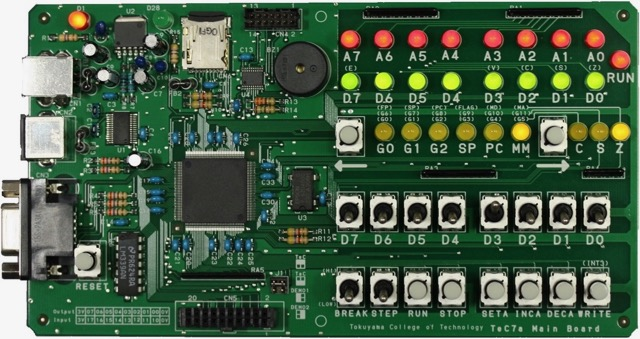
\includegraphics[scale=0.35]{Photo/TeC7.jpg}\\
(a) TeC7の写真
\end{center}
\end{minipage}
\begin{minipage}{0.38\columnwidth}
\begin{center}
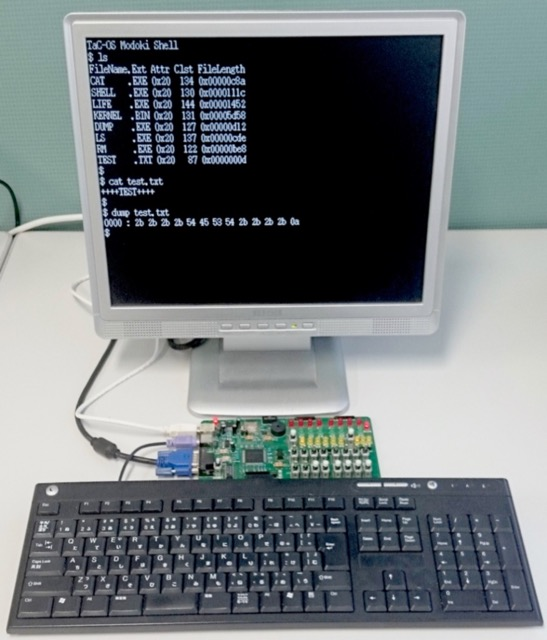
\includegraphics[scale=0.29]{Photo/TaC.jpg}\\
(b) TaCとしての使用例
\end{center}
\end{minipage}
\end{myfig}

TaC上では{\cmm}言語\footnote{
C言語に似た言語,
詳細は\url{https://github.com/tctsigemura/C--/blob/master/doc/cmm.pdf}を
参照のこと.}で記述されたTacOS\footnote{
詳細は\url{https://github.com/tctsigemura/TacOS}を参照のこと.} が動作する.
本書ではTacOSをオペレーティングシステムの実装例として参照する.

\subsection{ハードウェア構成}
\figref{tacBlock}にTaCのハードウェア構成を示す.
16ビットのシングルプロセッサ(CPUが一つ),
主記憶64KiBの非常に単純なシステムである.
単純なのでオペレーティングシステムの構築も容易である.
TaCに関する資料を付録\ref{appTac}にまとめる.

\myfigure{btp}{scale=0.48}{Fig/tacBlock-crop.pdf}
{TaCのハードウェア構成}{tacBlock}

\begin{itemize}
\item {\bf コンソールパネル} \\
\figref{tacPhoto}「(a) TeC7の写真」で,
TeC7本体右半分のランプやスイッチで構成される部分をコンソールパネルと呼ぶ.
コンソールパネルはCPUや主記憶と直接接続されており,
CPUを停止した状態で,
CPUや主記憶の内容を操作したり観察したりすることができる.
また,機械語命令を一命令毎に実行するステップ実行機能や,
ある番地の命令を実行した時点でプログラムを停止する
ブレーク機能ポイントが利用できる.
コンソールパネルの機能はハードウェアで実現されているので,
オペレーティングシステムの内部をステップ実行することも可能である.
TacOSの開発では,コンソールパネルがデバッグに活用された.

\item {\bf CPU} \\
\figref{tacRegPsw}に示すようなCPUレジスタとPSWを持つ16ビットCPUである.
PSWのフラグに実行モードを表すPビットを持ち,
カーネルモードとユーザモードを切り換えることができる.
機械語命令は,\figref{tacInsTbl}に示す46種類が準備されている.
機械語命令のアドレッシングモードは8種類ある.

\item {\bf メモリ} \\
メモリは\figref{tacMap}に示す構成である.
メモリ空間全体で64KiB,
自由に使用できるメモリが56KiB,
2KiBのVRAMと4KiBのIPL,32Bの割込みベクタからなる.
メモリは8ビット単位,または,16ビット単位で読み書きできる.
16ビット単位の場合は偶数アドレスを用いる.

\item {\bf タイマー} \\
$1$ミリ秒から$2^{16}-1$ミリ秒までの間隔で割込みを発生する
インターバルタイマーが二つ利用可能である.

\item {\bf ディスプレイアダプタ} \\
80文字×24行の文字をVGAディスプレイに表示する.
メモリ空間の{\tt E000h}から配置されるVRAMに書き込んだ
ASCIIコードと対応する文字をディスプレイに表示する.
{\tt E000h}番地がディスプレイの左上隅に対応する,
{\tt E001h}番地が一行目の2文字の位置,
{\tt E04Fh}番地が一行目の80文字の位置,
{\tt E050h}番地が二行目の1文字の位置に対応する.

\item {\bf SPIホストコントローラ} \\
スロットに挿入されたμSDカードをSPIモードに切換え読み書きを行う.
SPIホストコントローラに初期化コマンドを発行すると,
μSDカードをSPIモードに切換える.
ブロックアドレスとメモリアドレスを設定して読み出しコマンドを発行すると,
μSDカードの指定したブロックから512バイトのデータを
CPUを介さずに(DMA:Direct Memory Accessを用いて)メモリに読み出す.
書込みコマンドを発行すると,
メモリから指定ブロックにデータを書き込む.

\item {\bf シリアル通信インタフェース} \\
調歩同期方式,9,600Baudの通信インタフェースである.
USBシリアル変換ICを通してPC等のシリアルターミナルと通信できる.
1バイト転送する毎に割込みを発生する.

\end{itemize}

\subsection{TacOS}
\myfigure{btp}{scale=0.66}{Fig/tacosOrganization-crop.pdf}
{TacOSの構成}{tacosOrganization}

\figref{tacosOrganization}にTaC用のOSであるTacOSの構造を示す.
マイクロカーネルがプロセス間通信(IPC)機能を提供し,
サーバプロセスがメモリ管理やファイルシステム機能を提供する.
\figref{microkernel}の一般的なマイクロカーネル方式と異なり,
サーバプロセスがカーネルモードで動作しハードウェアに直接アクセスする.
また,サーバプロセスはマイクロカーネルと同じアドレス空間で動作するので,
カーネル内ルーチンをCALL機械語命令で直接に呼び出すことができる.

割込みやSVC命令の実行が原因で,
ユーザプロセスはカーネルモードに切り換わり
マイクロカーネル内の割込みハンドラが呼び出される.
割り込みハンドラで割込み原因を判断し,
マイクロカーネル内のルーチンを呼び出したり,
サーバプロセスの機能をIPCを用いて呼び出したりする.

\section{もう一つの仮想マシン}

\ref{osRole}で述べたように,
オペレーティングシステムは抽象化され便利な拡張マシン(仮想マシン)を,
必要な数だけ提供する.
ここで述べた仮想マシンは,単一ユーザ・プロセスの実行環境のことである.
同じ「仮想マシン」と言う用語が,
オペレーティングシステムを実行することが可能な,
よりハードウェアを忠実に再現した仮想マシンを指す場合もある.
ここでは,
一台のコンピュータ上で複数のオペレーティングシステムを実行可能な,
もう一つの仮想マシンについて紹介する.

\subsection{Type 2 ハイパーバイザ}
例えば,
Macを使用している人がWindowsでしか動作しないアプリケーションを使用する
場合を想像してしてみる\footnote{
徳山高専情報電子工学科のパソコン室では,
WindowsやLinuxでしか動作しないXilinx ISE WebPACKをMacで使用している.}.
予めMacのハードディスクにmacOSとは別にWindowsもインストールしておき,
電源投入時にmacOSとWindowsを選んでブートする方法もあるが,
オペレーティングシステムを切換える度にコンピュータを再起動するのは不便である.
また,macOSのアプリケーションとWindowsのアプリケーションを同時に実行したい
場合もある.

そこで,\figref{type2Hypervisor}に示すような
「Type 2 ハイパーバイザ(Type 2 Hypervisor)」を用いた仮想化が用いられる.
ハイパーバイザは
{\bf ホスト・オペレーティングシステム}の一つのユーザプロセスとして実行され,
コンピュータ一台の機能をエミュレーションする.
ハイパーバイザがエミュレーションするコンピュータの中で,
{\bf ゲスト・オペレーティングシステム}が稼働する.
エミュレーションはソフトウェアだけで完全に行うのではなく\footnote{
完全にソフトウェアで行う場合もある.},
ハードウェアの支援を受けて行うので高速に行うことができる\cite{virtualization}.
Type 2 ハイパーバイザとして有名は製品は,
VMware Workstation,
VMware Fusion,
VirtualBox\footnote{
徳山高専情報電子工学科のパソコン室では
macOS上のVirtualBoxでWindowsを動作させている.
%このWindowsの中でXlinix ISE WebPACKが使用できる.
}等である.

\myfigure{btp}{scale=0.66}{Fig/type2Hypervisor-crop.pdf}
{Type 2 ハイパーバイザ}{type2Hypervisor}

\subsection{Type 1 ハイパーバイザ}
メインフレーム上で1960年代から使用されている方式である.
現在ではPCサーバの仮想化にも使用されている.
Type 1 ハイパーバイザはホスト・オペレーティングシステム無しに
ハードウェア上で直接実行される.
Type 1 ハイパーバイザとして有名な製品は,
IBM z/VM,
VMware vSphere,
Xen,
Hyper-V等である.

サーバ向けの製品が主流であり,
例えば VMware vSphere は
実行中のゲストを他の物理サーバに移動する等,
非常に高度な機能を持っており\cite{vsphere},
一台のサーバ上に効率よく多数の仮想マシンを動かすことができる.
徳山高専情報電子工学科のパソコン室でも,
2台のサーバ上に50台の仮想デスクトップマシンを動かしていたことがある.

\myfigure{btp}{scale=0.66}{Fig/type1Hypervisor-crop.pdf}
{Type 1 ハイパーバイザ}{type1Hypervisor}

\subsection{仮想アプライアンス}
ゲスト・オペレーティングシステムとアプリケーションまでインストールし,
すぐに使用できる状態で配布される仮想マシンである.
例えば,メールフィルタソフトをインストールした仮想マシンを
入手しハイパーバイザで実行するだけですぐにメールフィルタリングが開始できる.

同じ手法で,
すぐに使用できるパーソナルコンピュータ用の
デスクトップ・オペレーティングシステムが配布されている場合もある.
Linux の一種であるUbuntuの場合,
VirtulBoxですぐに実行できるディスクイメージがダウンロードできる\cite{ubuntu}.
仮想アプライアンスは,
ソフトウェアの新しい流通手法である.

\section{まとめ}
本書は{\bf SMP(対称型マルチプロセッシング:Symmetric Multiprocessing)}の
コンピュータを前提にしている.
CPUは{\bf PSW(Program Status Word)}と{\bf CPUレジスタ}を含んでいる.
最近のIntel社のCPUでは,従来のCPUを{\bf Core(コア)},
複数のコアを含んだLSIのことをCPUと呼ぶ.

オペレーティングシステムのカーネルは,
割込みハンドラ,ディスパッチャ,サービスモジュール,
デバイスドライバ等から構成される.
ユーザ・プロセスからカーネルへの切換え原因は{\bf 割込み}だけである.
ユーザ・プロセス毎に{\bf 仮想CPU},{\bf 仮想メモリ空間},管理情報等を
持っている.

カーネルの構成方式には,
{\bf 単層カーネル(モノリシック・カーネル)}方式と
{\bf マイクロカーネル(micro-kernel)}方式の二種類があった.
マイクロカーネル方式ではサービスモジュールをサーバ・プロセスとし,
{\bf IPC(プロセス間通信)}を用いてサービスを要求する.
サービスモジュール間の独立性が高くなり高信頼性のシステムを構成可能であるが,
IPCはオーバーヘッドが大きい.
信頼性と性能はトレードオフの関係にある.

{\bf TaC}は,本書でオペレーティングシステムの実装例として使用する
TacOSを稼働させるコンピュータである.
コンソールパネルを持ち,
TacOSのカーネル内までステップ実行によるトレースが可能である.
{\bf TacOS}はマイクロカーネル方式の簡単なオペレーティングシステムである.
本書では,しばしばTacOSのソースコードを実装例として参照する.




 % 前提知識
\chapter{CPUの仮想化}
オペレーティングシステムは,
ハードウェアを抽象化した使いやすい拡張マシン(仮想マシン)を
必要な数だけ提供する.
数に限りがある資源は,必要な数だけあるように見せるために仮想化が行われる.
CPU資源も仮想化し,各プロセスが自分専用のCPUを持っているように見せかける.

%==============================================================================
\section{時分割多重}
CPUを仮想化するためには時分割多重が用いられる.
ハードウェアである実CPUの数は限られているので,
時間を区切って実CPUを使用するプロセスを次々に切換えていく.
\figref{virtualCPU}にCPU仮想化の原理を示す.

\begin{myfig}{btp}{時分割多重によるCPUの仮想化}{virtualCPU}
  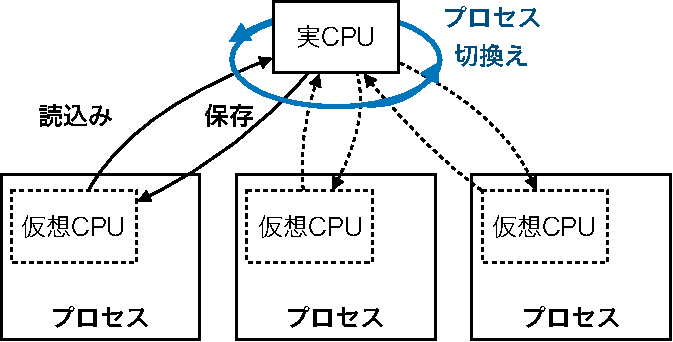
\includegraphics[scale=0.7]{Fig/virtualCPU-crop.pdf}
\end{myfig}

実CPUは\figref{cpuBlock}のような構造をもつハードウェアである.
プロセスの構造は\figref{procOrganization}に示した通りであり,
仮想CPUを含んでいる.
実CPUが短時間(例えば10ms)に次々と実行するプロセスを切換えていくことで,
複数のプロセスが夫々に専用のCPUを持ち並行して実行されているように見せかける.

CPUが実行するプロセスを切り換えるには,まず,
実CPUのコンテキストを現在のプロセスの仮想CPU領域に保存する.
次に,新しく実行するプロセスの仮想CPU領域から実CPUにコンテキストを読込み,
新しいプロセスの実行を再開する.
一つのプロセスから別のプロセスに切換える処理を
\emph{コンテキストスイッチ}と呼ぶ.
また,実CPUにコンテキストを読込んで実行を再開することを\emph{ディスパッチ},
ディスパッチを行うプログラムを\emph{ディスパッチャ}と呼ぶ.
\figref{osOrganization}にもディスパッチャは描かれていた.

%==============================================================================
\section{プロセスの状態}
\label{procState}
プロセスは,
キーボード等の入出力装置からの入力を待つ状態になったり,
時間が経過するのを待つ状態になったりする.
\emph{待ち(Waiting)状態}のプロセスにはCPUを割当てる必要がない.
このようにプロセスは幾つかの状態を持っている.
プロセスの状態はUNIXではpsコマンドで確認できる.
プロセスを模式的に示した\figref{procOrganization}では,
「プロセス情報」の「プロセスの状態」のことである.

\subsection{基本的な三つの状態}
\figref{procState}にプロセスの状態遷移図を示す.
この図は最も簡単なものであり,
実際のオペレーティングシステムでは,
もっと状態数が多くなる\footnote{
  macOSのpsコマンドのオンラインマニュアルで確認すると,
  macOSではプロセスの状態が,
  I(Idle),
  R(Runnable),
  S(Sleep),
  T(sTopped),
  U(Uninterruptible wait),
  Z(Zombie)の六つであることが分かる.}.
図に示された三つの状態を説明する.

\begin{itemize}
\item \emph{Ready(実行可能)} \\
  CPUを割当てれば実行を開始できる状態のことである.
  プロセスはCPUが割当てられるのを待っている.
\item \emph{Running(実行中)} \\
  CPUが割当てられ実行している状態のことである.
  CPUの数より多くのプロセスが同時にRunningになることはできない.
\item \emph{Waiting(待ち)} \\
  シグナルの到着や入出力の完了等の事象(イベント)を待っている状態である.
  プロセスは実行することができない.
\end{itemize}

\begin{myfig}{btp}{プロセスの状態遷移}{procState}
  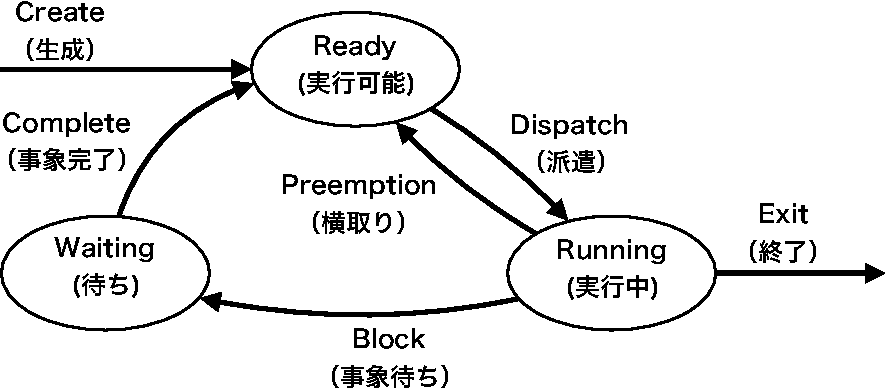
\includegraphics[scale=0.66]{Fig/procState-crop.pdf}
\end{myfig}

\subsection{状態遷移}
\figref{procState}に示された六つの状態遷移の意味は以下の通りである.

\begin{enumerate}
\item \emph{Create(クリエート,生成)} \\
  新しいプロセスが生成されるとReady状態になる.
  親プロセスが\|fork()|システムコール(UNIXの場合)や
  \|CreateProcess()|システムコール(Windowsの場合)を実行すると,
  新しい子プロセスが生成される.
\item \emph{Dispatch(ディスパッチ,派遣)} \\
  Ready状態のプロセスは,
  自分の順番が来たらCPUが割当てられRunning状態に遷移し実行を開始する.
\item \emph{Preemption(プリエンプション,横取り)} \\
  Running状態のプロセスは,
  決められた時間(クオンタムタイム)を使い切ったときや,
  より優先度の高いプロセスがReady状態になったとき,
  CPUを取り上げられReady状態に遷移する.
\item \emph{Block(ブロック,事象待ち)} \\
  Running状態のプロセスが,
  システムコールを発行して自らWaiting状態に遷移することがある.
  例えば入出力システムコール
  (\|open()|,\|read()|,\|write()|,\|close()|等)や,
  シグナル待ちシステムコール(\|pause()|,\|wait()|,\|sleep()|等)
  を発行した場合である.
  また,他のプロセスからシグナルを受信した場合も,
  Waiting状態に遷移することがある.
  更に,仮想記憶の機能を持つオペレーティングシステムでは,
  プロセスが読み書きしようとした領域がメモリ上に存在しない時も
  この遷移が起こり,
  メモリ領域を確保するための処理がカーネル内部で始まる.
\item \emph{Complete(コンプリート,事象完了)} \\
  Waiting状態のプロセスは,
  入出力の完了やシグナルの発生等の事象(イベント)が発生すると
  Ready状態に遷移する.
  Waiting状態のプロセスは停止しているのでプロセスが事象を発生することはない.
  事象はプロセスの外部からもたらされる.
\item \emph{Exit(終了)} \\
  プロセスが自ら\|exit()|システムコール(UNIXの場合)や
  \|ExitProcess()|システムコール(Windowsの場合)を用いて終了する場合,
  または,プロセスがシグナルを受ける等して終了させられる場合に,
  この遷移が起こる.
  シグナルはプロセス(他プロセス,自プロセス)から明示的に送信される場合と,
  自プロセスが保護違反などのエラーを起こして発信される場合がある.
\end{enumerate}

%==============================================================================
\section{プロセスの切換え(コンテキストスイッチ)}
Running状態のプロセスがBlock遷移またはPreemption遷移しCPUを取り上げられると,
他のReady状態のプロセスがCPUを割付けられDispatch遷移し実行を再開する.

\subsection{切換えの原因}
Running状態のプロセスが状態遷移を起こす原因を以下にまとめ直す.

\begin{enumerate}
\item イベント \\
  Running状態のプロセスは,
  自ら「システムコールを発行」することでBlock遷移をすることがある.
  また,他のプロセスからの「\emph{干渉}\footnote{
      干渉には,より優先順位の高いプロセスが実行可能になった,
      別のプロセスからシグナル等を受取った等がある.}
    を受け」Block遷移することがある.
\item タイムスライシング \\
  Running状態のプロセスが長時間の実行を続けるとPreemption遷移をする.
  一度に実行しても良い時間(クオンタムタイム)を使い切ったためである.
  Ready状態のプロセスが他にあれば,そのプロセスに実行が切換わる.
  他に実行すべきプロセスが無い場合は,再度,同じプロセスが実行される.
\end{enumerate}

\subsection{切換え手順}
\figref{procSwitch}に二つのプロセス間で実行が切り換わる様子を示す.
図では時間に従って上から下へ処理が進む.
左側はプロセスAの実行を,
右側はプロセスBに実行を,
中央はカーネルの実行を表している.
以下では,
図の上半分でプロセスAからプロセスBに実行が切り替わる手順を説明する.
図の下半分の説明は省略するが,
上半分と同様な手順でプロセスBからプロセスAに切り替わる手順を示している.

\begin{myfig}{btp}{プロセスの切換え}{procSwitch}
  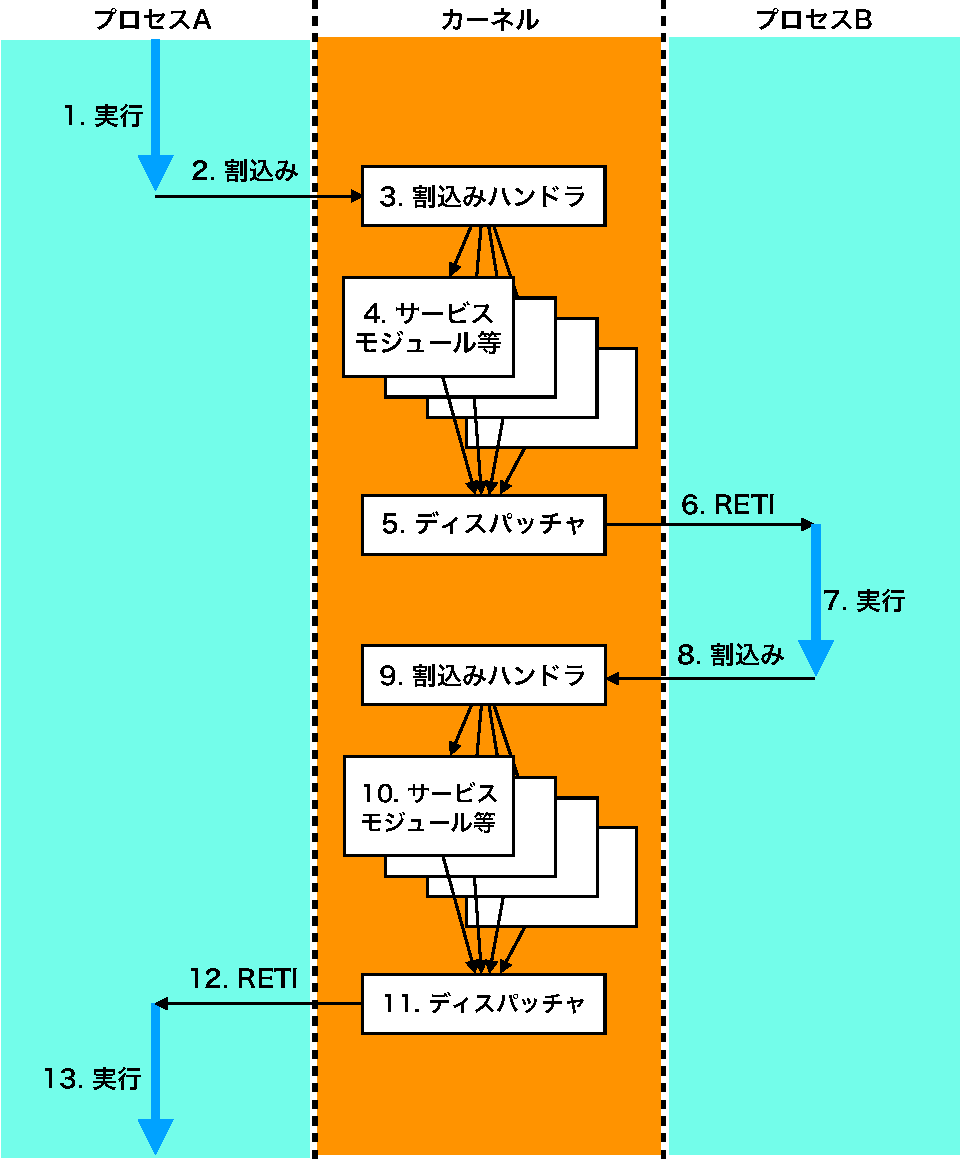
\includegraphics[scale=0.6]{Fig/procSwitch-crop.pdf}
\end{myfig}

\begin{enumerate}
\item 実行 \\
  日頃はCPUがユーザ・プロセスを実行している.
\item 割込み \\
  割込みが発生し処理がプロセスAからカーネル内の割込みハンドラに移る.
  割込みの原因は\ref{interruptSource}で述べた様々なものが考えられる.
  割込みが発生すると以下の処理が\emph{CPUのハードウェアにより自動的に}される.
  \begin{enumerate}
  \item CPUの(PCを含む)PSWがスタックに保存される.
  \item CPUの実行モードがカーネルモードに切り換わる.
  \item 割込みハンドラにジャンプする.
  \end{enumerate}
\item 割込みハンドラ \\
  PSW(スタック上にある)とCPUレジスタ(\figref{cpuBlock}参照)からなる
  プロセスのコンテキストを
  プロセスの仮想CPU領域(\figref{procOrganization}参照)に保存する.
  次に割込み原因を調べ,
  割込み原因に応じた処理(サービスモジュール等)にジャンプする.
  例えば,
  割込み原因が\|open()|システムコールなら,
  openシステムコールの処理を行うファイルシステムの
  サービスモジュールにジャンプする.
  割込み原因がI/O完了なら,
  完了したI/Oに対応するデバイスドライバにジャンプする.
\item サービスモジュール等 \\
  サービスモジュールやデバイスドライバが割込み原因に応じた処理を行う.
  この過程でプロセスの状態が変化することがある.
  例えば,プロセスが発行したシステムコールが原因でBlock遷移する場合や,
  タイマーやI/Oの完了割込によりWaiting状態だった別のプロセスが
  Complete遷移する場合,
  タイマーの完了割込により現在のプロセスがPreemption遷移する場合等が
  考えられる.
  サービスモジュール等の処理が完了するとディスパッチャにジャンプする.
\item ディスパッチャ \\
  実行可能なプロセスの中から一つを選び,
  選んだプロセスの仮想CPU領域の内容をCPUレジスタにロードする.
  最後にPSWを復旧する機械語命令(RETI)を実行しプロセスの実行に戻る.
\item RETI \\
  PSWを復旧する機械語命令として
  割込復帰用の\emph{RETI(RETurn from Interrupt)命令}を用いる.
  RETI命令は単一の命令でPSW(PCとフラグ)を一度にスタックから復旧する.
  CPUの実行モードを表すフラグはPSWに含まれているので,
  PSWが復旧されることで実行モードがカーネルモードからユーザモードに切り換わる.
\item 実行 \\
  新しく選択されたユーザ・プロセスが実行される.
\end{enumerate}

\subsection{切換えの例}
計算に長い時間を要する二つのプロセスだけがある時,
クオンタムタイムを使い切ってもう一方のプロセスに切り換わり,
交互に実行される様子を\figref{procSwitchInst}に示す.
以下に手順を説明する.

\begin{myfig}{btp}{プロセスの切換えの例}{procSwitchInst}
  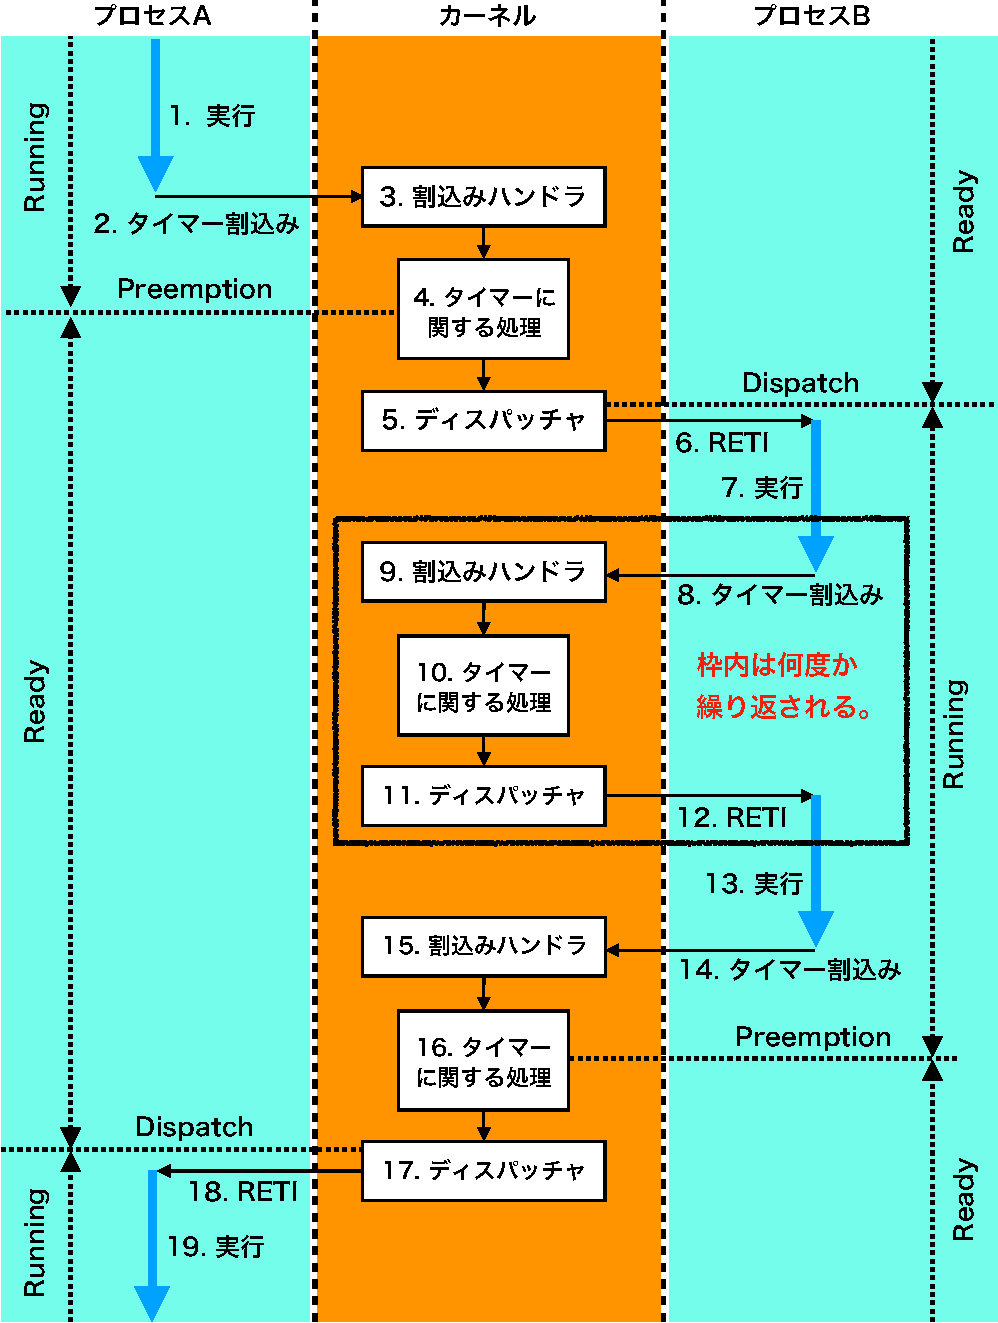
\includegraphics[scale=0.6]{Fig/procSwitchInst-crop.pdf}
\end{myfig}

\begin{enumerate}
\item 実行 \\
  プロセスAは計算処理を続けている.
  長い時間に渡ってシステムコールを発行することは無い.
\item タイマー割込み \\
  タイマーは一定間隔で割込みを発生する.
  割込が発生するとCPUのハードウェアが自動的にPSWを保存し,
  割込みハンドラにジャンプする.
  オペレーティングシステムは,
  主に,この割込みを基準に時間の経過を認識する.
\item 割込みハンドラ \\
  プロセスのコンテキストをプロセスの仮想CPUに保存する.
  その後,割込原因を調べタイマーからの割込みなので,
  「タイマーに関する処理」を行うカーネル内のモジュールへジャンプする.
\item タイマーに関する処理 \\
  一定間隔で発生するタイマーからの割込みを利用して,
  システムの時計を進めたり,
  リソース(CPUやメモリ等)の利用統計データを更新したりする.
  その間にプロセスAがクオンタムタイムを使い切ったことが判明すると,
  プロセスAをPreemption遷移させる.
  この時点でプロセスAの状態がReadyに変化する.
\item ディスパッチャ \\
  Ready状態のプロセスの中から適切な一つを選びDispatch遷移させる.
  \figref{procSwitchInst}はプロセスBが選択された場合である.
  ディスパッチャはプロセスBのCPUレジスタを復旧する.
\item RETI \\
  プロセスBのPSWを復旧し,プロセスBの実行を再開する.
\item 実行 \\
  プロセスBは計算処理を再開する.
  プロセスBも長い時間計算を続けるプロセスとする.
\item タイマー割込み \\
  計算を続けるうちにタイマーからの割込みが発生する.
\item 割込みハンドラ \\
  プロセスBのコンテキストを保存する.
\item タイマーに関する処理 \\
  プロセスBは,まだ,クオンタムタイムを使い切っていないので,
  Preemptionは発生しない.
\item ディスパッチャ \\
  Preemptionは発生しないので,
  プロセスBのコンテキストを復旧する.
\item RETI \\
  プロセスBに戻る.
\item 実行 \\
  プロセスBは計算処理を再開する.
\item タイマー割込み \\
  8.〜13. を何度か繰り返し,
  クオンタムタイムを使い切った時のタイマー割込みである.
\item 割込みハンドラ \\
  プロセスBのコンテキストを保存する.
\item タイマーに関する処理 \\
  クオンタムタイムを使い切ったのでPreemptionが発生する.
\item ディスパッチャ \\
  Ready状態のプロセスAを選択しDispatch遷移させる.
  プロセスAのコンテキストを復旧する.
\item RETI \\
  プロセスAに戻る.
\item 実行 \\
  プロセスAは計算処理を再開する.
\end{enumerate}

%==============================================================================
\section{PCB(Process Control Block)}
PCBはプロセスを表現する重要なカーネル内のデータ構造である.
PCBはカーネル内のプロセステーブルに格納される.

\subsection{PCBの内容}
PCBは,\figref{procOrganization}の
「仮想CPU」と「プロセス情報」を合わせたものに相当する.
PCBには以下のような情報が格納される.

\begin{itemize}
\item 仮想CPU
\item プロセス番号
\item 状態(Running,Waiting,Ready等)
\item 優先度
\item 統計情報(CPU利用時間等)
\item 次回のアラーム時刻
\item 親プロセス
\item 子プロセス一覧
\item シグナルハンドリング
\item 使用中のメモリ
\item オープン中のファイル
\item カレントディレクトリ
\item プロセス所有者のユーザ番号
\item PCBのリストを作るためのポインタ
\end{itemize}

\subsection{PCBリスト}
カーネル内ではPCBがプロセスを表現する.
例えば,優先順にソートされたReady状態のプロセスのリストは,
優先度をキーにソートされたPCBの線形リスト(\emph{待ち行列})として表現される.
この線形リストを\emph{実行可能列}と呼ぶ.
その様子を\figref{procQueue}に示す.
図は,数値が小さいほど優先度が高い意味になっている.

\begin{myfig}{btp}{PCBのリスト}{procQueue}
  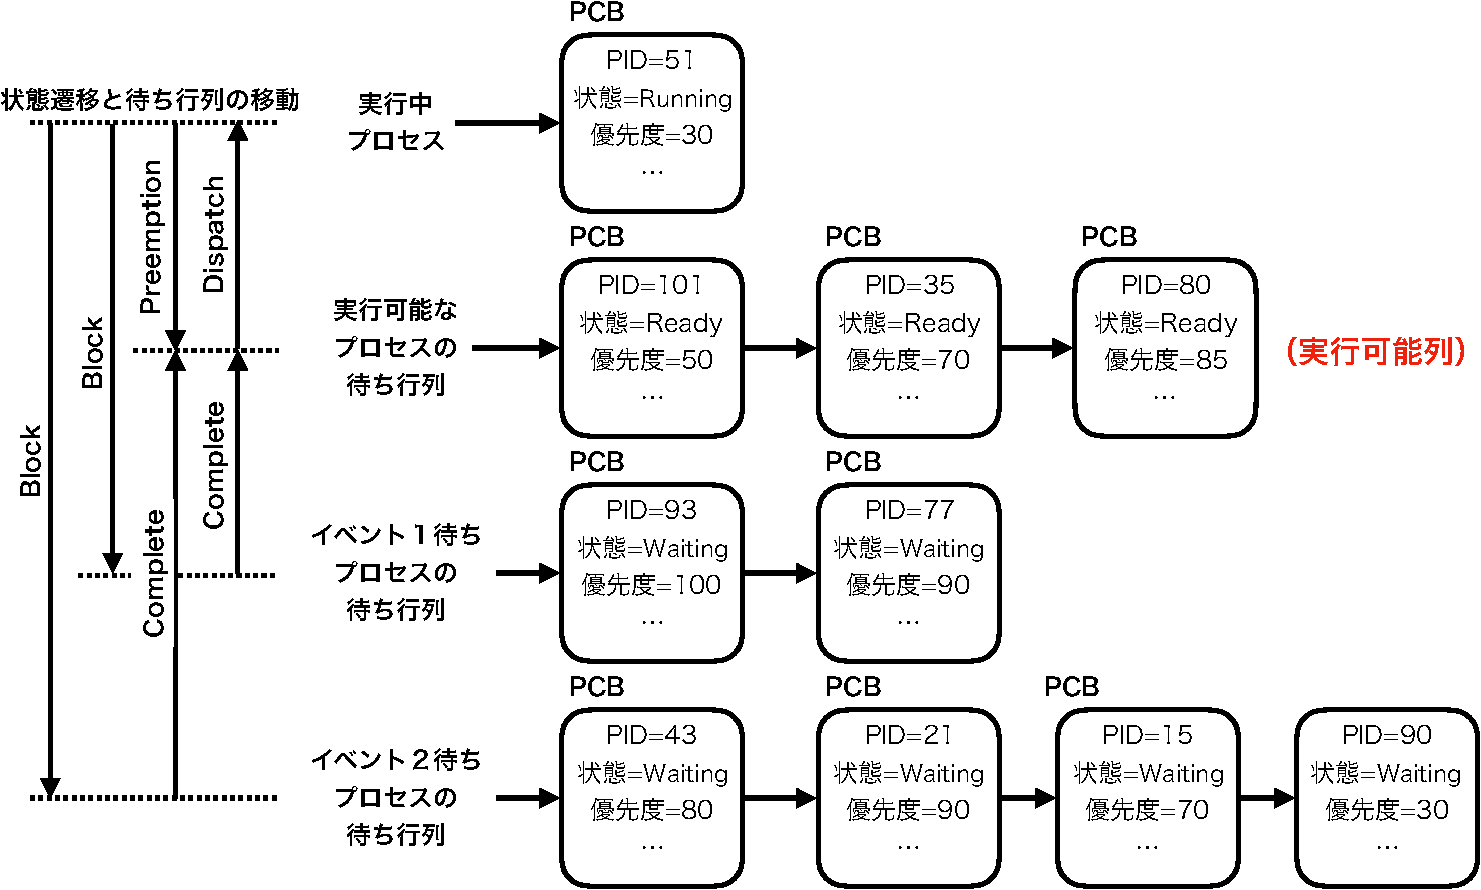
\includegraphics[scale=0.55]{Fig/procQueue-crop.pdf}
\end{myfig}

Ready状態のプロセスだけでなく,
Running状態のプロセスや,
Waiting状態のプロセスも待ち行列で管理される.
Waiting状態のプロセスは,
待ち合わせているイベント毎に待ち行列を作っている.
イベント待ち行列のソート順はイベント毎にルールが決められる.

プロセスの状態遷移に合わせてPCBが待ち行列の間を移動する.
\figref{procQueue}の左側の「状態遷移と待ち行列の移動」が
「どの待ち行列から,どの待ち行列に移動可能か」を表している.
例えば,Running状態(実行中)のプロセスがPreemption遷移をすると,
状態がReadyに変わるだけでなく,
PCBが「実行可能なプロセスの待ち行列」に移動する.
この移動ルールは\figref{procState}の状態遷移と一致している.

%==============================================================================
\section{スレッド(Thread)}
ここまで,一つのプロセスが一つの仮想CPUを持つモデルを考えてきた.
しかし,実際のコンピュータハードウェアはCPUを複数持つSMPの場合もある.
これでは
「ハードウェアの機能を抽象化した便利な\emph{拡張マシン}」
(\ref{abstruction}参照)であるはずのプロセスが,
「CPUが一つしかない\emph{縮小マシン}」なっている.
そこで,SMPに対応しプロセスが複数の仮想CPUを持つモデルを導入する.
これにより,一つのプロセスが
並列実行する複数の処理の流れ(スレッド)を持つことが可能になる.

\subsection{スレッドの役割}
複数のプロセス(ジョブ)を主記憶にロードしておくことで
CPUの利用効率を高くできることは既に説明した
(\pageref{multiprogramming}ページ,マルチプログラミング参照).
マルチプログラミングの,もう一つのメリットは,
プログラミングが簡単になる場合があることである.
以下ではWebサーバを例に,
マルチプログラミングによる改善を紹介する.

\begin{itemize}
\item マルチプロラミングなし \\
  \figref{singleProcSingleClient}に最も簡単なモデルを示す.
  Webサーバはリクエストを受信すると,それに対するレスポンスを返す.
  処理は1番目のクライアントから順に行われ,
  2番目のクライアントは1番目の処理が終了するまで待たされる.
  このモデルの問題点は,
  処理中にWebサーバプロセスがI/O待ち等でブロック(Block)する可能性があり,
  その間,他のクライアントへのサービスがされないことである.

  2番目以降のクライアントが長時間待たされないように,
  複数のクライアントの処理を並行してできるように改良したモデルが
  \figref{singleProcMultiClient}である.
  「I/O完了の監視」は通信を含む複数の入出力を同時に監視し,
  どれかが読み書き可能になるのを待つ機能である.
  UNIXでは\|select()|システムコールがこの機能を持つ.
  読み書き可能になったことを確認後に読み書きを行うので
  プロセスがブロックすることが無くなり,
  複数のクライアントに対して同時にサービスを行うことができる.

  しかし,Webサーバのプログラミングは難しくなる.
  一方のクライアントの処理が終わらないうちに,
  別のクライアントの処理を開始する必要があるからである.
  クライアント毎に処理がどこまで進んでいるのかを表す
  \emph{状態}を持つ必要がある.
  また,CPUが複数存在する場合でも,
  同時には一つのCPUしか働かないことも問題である.

  \begin{myfig}{btp}{マルチプログラミングを用いないWebサーバ}
    {singleProcSingleThread}
    \begin{minipage}{0.49\columnwidth}
      \begin{center}
        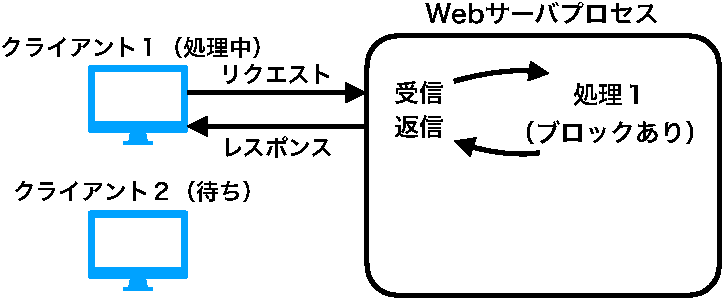
\includegraphics[scale=0.6]{Fig/singleProcSingleClient-crop.pdf}
        \subcaption{最も基本的なWebサーバのモデル}
        \label{fig:singleProcSingleClient}
      \end{center}
    \end{minipage}
    \begin{minipage}{0.49\columnwidth}
      \begin{center}
        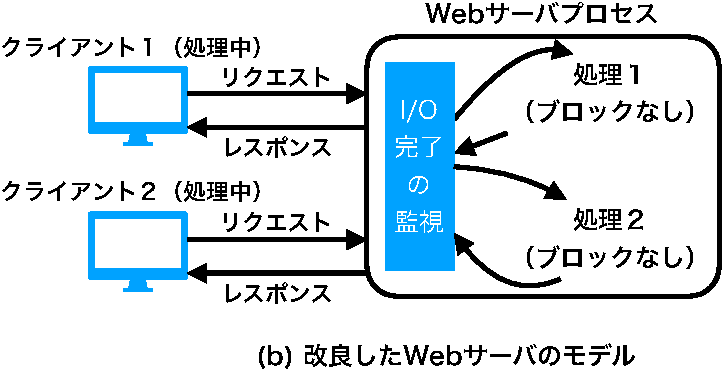
\includegraphics[scale=0.6]{Fig/singleProcMultiClient-crop.pdf}
        \subcaption{改良したWebサーバのモデル}
        \label{fig:singleProcMultiClient}
      \end{center}
    \end{minipage}
  \end{myfig}
  
\item マルチプロセス \\
  マルチプログラミングを用いることで前記の問題を解決したモデルを
  \figref{multiProc}に示す.
  Webサーバプロセスは,
  まず,接続要求を待ちクライアント1からの接続を受け入れる.
  次に,クライアント1専用のサーバプロセスを生成し処理を任せる.
  Webサーバプロセスは,
  生成したプロセスの終了を待たずに,
  次の接続要求待ちになる.
  クライアント2からの接続要求があったら
  クライアント2専用のサーバプロセスを生成し,
  接続要求待ちに戻る.

  このモデルなら,
  各クライアントの処理を別々のプロセスが行っているので,
  プロセスがブロックしても構わない.
  そのため,プログラミングは簡単になる.
  また,CPUが複数あればプロセスが真に並列に実行される.
  しかし,プロセスの生成はメモリ空間の確保や初期化を含み\emph{重い処理}である.
  また,
  プロセスはメモリを共有していないのでプロセス間の情報共有には効率が悪い.

\item マルチスレッド \\
  複数のスレッドを使用したモデルを\figref{multiThread}に示す.
  マルチプロセスの場合と良く似たプログラムであるが,
  クライアント毎に専用のプロセスを作る代わりに,
  クライアント毎に専用のスレッドを作る.
  スレッドの生成はプロセス生成より10〜100倍速いと
  言われている\cite{lightWeight}.
  また,スレッドはメモリを共有しているので情報共有には都合が良い.
  例えば,Webサーバが頻繁に参照されるページをメモリ上にキャッシュする場合,
  キャッシュをスレッドで共有できる.

  \begin{myfig}{btp}{マルチプログラミングを用いるWebサーバ}{multiPrograming}
    \begin{minipage}{0.49\columnwidth}
      \begin{center}
        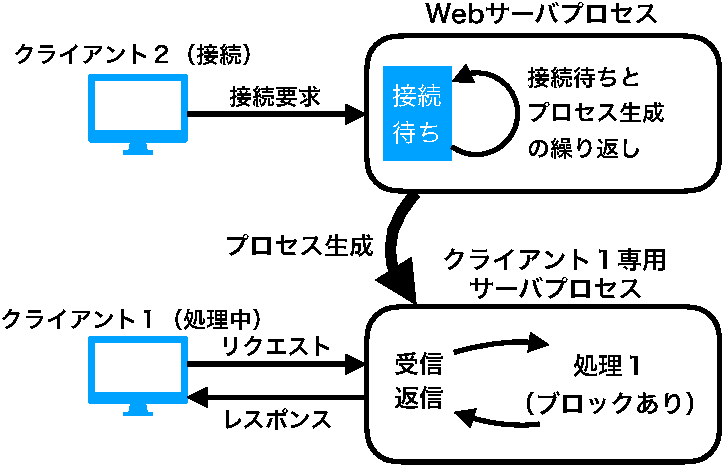
\includegraphics[scale=0.6]{Fig/multiProc-crop.pdf}
        \subcaption{マルチプロセスにしたWebサーバのモデル}
        \label{fig:multiProc}
      \end{center}
    \end{minipage}
    \begin{minipage}{0.49\columnwidth}
      \begin{center}
        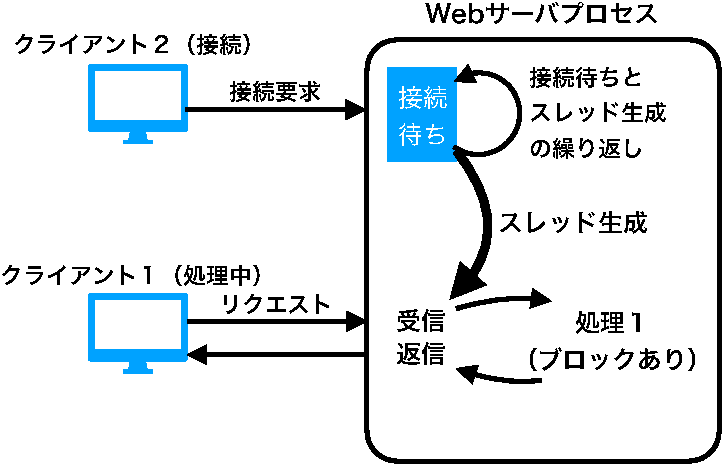
\includegraphics[scale=0.6]{Fig/multiThread-crop.pdf}
        \subcaption{改良したWebサーバのモデル}
        \label{fig:multiThread}
      \end{center}
    \end{minipage}
  \end{myfig}
\end{itemize}

\subsection{スレッドの形式}
読者は,「スレッドはカーネルが実現する」と暗黙のうちに考えていたかも知れない.
しかし,ユーザプログラム(ライブラリ)内でスレッドを実現することもある.
カーネルが実現するスレッドを\emph{カーネルスレッド},
ユーザプログラム内で実現するスレッドを\emph{ユーザスレッド}と呼ぶ.

\begin{myfig}{btp}{ユーザスレッドとカーネルスレッド}{threadOrganization}
  \begin{minipage}{0.49\columnwidth}
    \begin{center}
      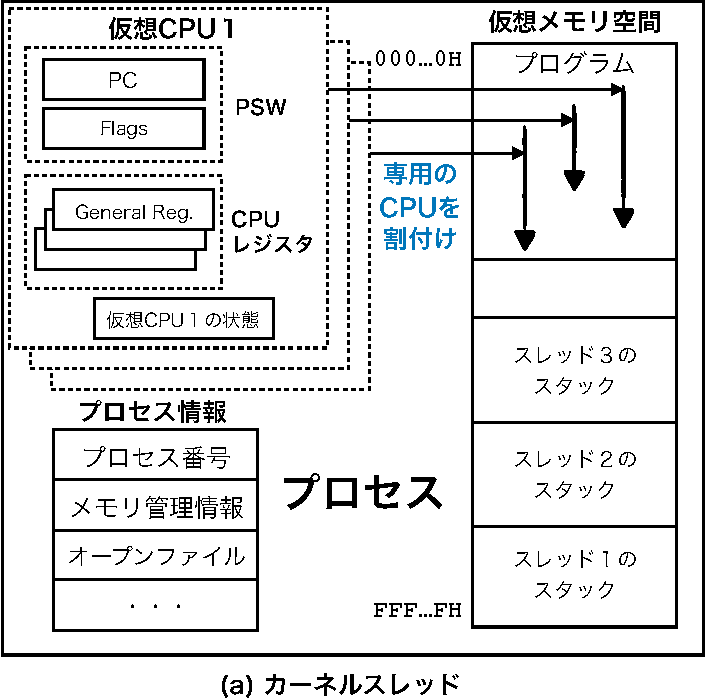
\includegraphics[scale=0.6]{Fig/kernelThread-crop.pdf}
      \subcaption{カーネルスレッド}
      \label{fig:kernelThread}
    \end{center}
  \end{minipage}
  \begin{minipage}{0.49\columnwidth}
    \begin{center}
      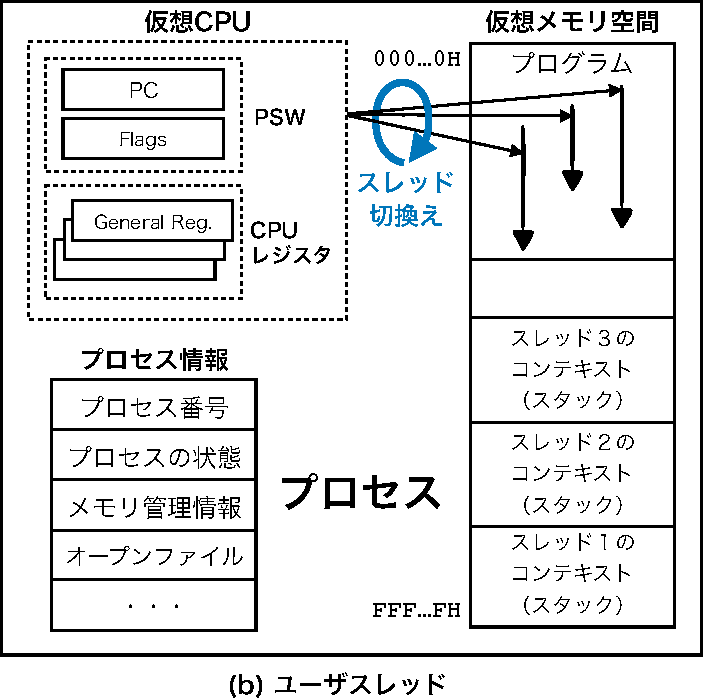
\includegraphics[scale=0.6]{Fig/userThread-crop.pdf}
      \subcaption{ユーザスレッド}
      \label{fig:userThread}
    \end{center}
  \end{minipage}
\end{myfig}

\begin{itemize}
\item \emph{カーネルスレッド} \\
  カーネルスレッドの模式図を\figref{kernelThread}に示す.
  カーネルスレッドはプロセスの仮想CPUを複数にし,
  仮想CPUがプログラムを並行して実行する.
  「プロセス情報」から「プロセスの状態」は無くなり,
  代わりに仮想CPU毎に「仮想CPUの状態」を管理するようになる.
  CPUが複数ある時,カーネルスレッドであれば,
  プロセス内を真に並列実行することが可能である.
\item \emph{ユーザスレッド} \\
  ユーザスレッドの模式図を\figref{userThread}に示す.
  プロセスには単一の仮想CPUしかない.
  ユーザスレッドは仮想CPUを時分割多重して実現される.
  カーネルを経由しないでスレッドの生成や切換えをすることができるので,
  オーバーヘッドが非常に小さい.
\end{itemize}

以下に述べるように,両者を組合せた三つのスレッドモデルが使用される.

\begin{enumerate}
\item \emph{One-to-One Model} \\
  全てのスレッドがカーネルスレッドのモデルである.
  \figref{kernelThread}に相当する.
  プロセス内にカーネルが管理する仮想CPUが複数あるので,
  複数プロセスと同等な並列実行が可能である.
  しかし,スレッドの生成や切換えにカーネルが介入するので,
  処理は重くなる.
  また,システムによっては生成できるスレッド数に制限がある.
\item \emph{Many-to-One Model} \\
  複数(Many)のユーザスレッドを
  一つ(One)のカーネルスレッドで実行するモデルである.
  \figref{userThread}に相当する.
  プロセス内にカーネルスレッドは一つしか存在しない.
  ユーザスレッドはユーザプログラム(ライブラリ)の工夫で
  単一のカーネルスレッドを複数に見せかけているだけなので,
  真の並列実行にはならない.
  また,何れかのスレッドがシステムコールでブロックすると,
  全てのスレッドが停止してしまう問題がある.
\item \emph{Many-to-Many Model} \\
  複数の(Many)のユーザスレッドを
  複数の(Many)のカーネルスレッドで実行するモデルである.
  カーネルスレッドの数をユーザスレッドの数より多くすることはない.
  前記二つのモデルの折衷案である.
\end{enumerate}

\subsection{スレッドプログラミング}
配列データの合計を求める処理をスレッドを用いて高速化する例を考えよう.
\figref{threadedSum}に原理を示す.
配列\|a|をM分割し個別スレッドで(CPUが複数あれば)同時に小計を計算する.
小計は配列\|total|に格納する.
最後に\|main|スレッドが\|total|の合計を求めると全体の合計\|sum|が計算できる.

\begin{myfig}{btp}{M個のスレッドで手分けして合計を計算する様子}{threadedSum}
  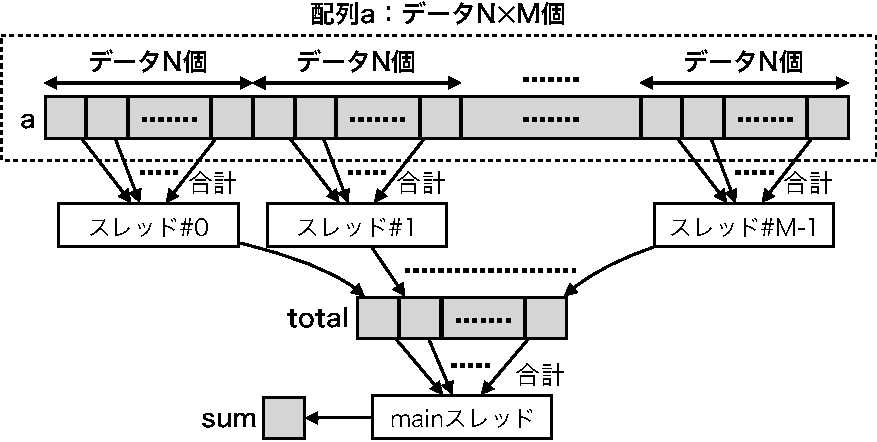
\includegraphics[scale=0.66]{Fig/threadedSum-crop.pdf}
\end{myfig}

\subsubsection{POSIXスレッドによる実装}
このアイデアをPOSIXスレッド\footnote{
  POSIXスレッドはUNIX系のオペレーティングシステムで使用できる.
}を用いたC言語プログラムにしたものをリスト\ref{threadTest}\footnote{
  このプログラムは macOS High Sierra で動作確認をした.
}に示す.

\lstinputlisting[numbers=left,float=btp,label=threadTest,
  caption=M個のスレッドで分担して配列データの合計を求めるプログラム]
  {SampleCode/pThread/threadTest.c}

12行の\|thread()|関数はM個のスレッドで同時に並列実行される.
配列\|a|の担当範囲等は引数\|arg|により指示される.
関数の引数(\|arg|)やローカル変数(\|args|,\|sum|,\|i|)は,
スレッドのスタック(\figref{threadOrganization}参照)に割付けられるので,
スレッド毎に別の実体を持つ.
グローバル変数\|a|や\|total|等は全てのスレッドで共有される.

32行の\|pthread_attr_init()|は引数の\|pthread_attr_t|型変数を
デフォルトのアトリビュート値で初期化する.
33行の\|pthread_create()|がスレッドを生成する関数である.
新しいスレッドの実行は引数で指定された\|thread()|関数から始まる.
\|pthread_create()|の引数\|p|は,
\|thread()|関数が実行を開始する時に\|arg|引数に渡される.

38行の\|pthread_join()|はスレッドの終了を待つ関数である.
スレッドの終了が確認できたら,39行で小計を\|sum|に足し込む.

\subsubsection{実行時間の計測結果}
リスト\ref{threadTest}のプログラムの実行時間を\tabref{threadTimeTbl}に,
グラフにしたものを\figref{threadTimeGrph}に示す
\footnote{
  実行時間の計測にはOS X の \texttt{time} コマンドを用いた.
}
\footnote{
  実行時間が短すぎて比較し難いので,
  プログラムの14行から17行を10万回繰り返すように改造した上で計測した.}
\footnote{
  計測に使用したコンピュータは
  OS X Yosemite をインストールした
  Mac Pro(Late 2013, 3.5GHz 6-Core Intel Xeon E5)である.
  %macOS High Sierra をインストールした
  %MacBook Pro(Retaina, 13-inch, Mid 2014, 2.8GHz Intel Core i5)である.
  C言語コンパイラは
  Apple LLVM version 7.0.0(clang-700.0.72)を使用した.
}.

\begin{mytable}{btp}{スレッド数による実行時間比較}{threadTimeTbl}
  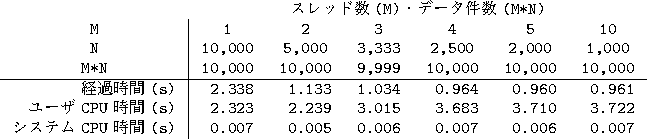
\includegraphics[scale=1.0]{Tbl/threadTimeTbl.pdf}
\end{mytable}

\begin{myfig}{btp}{スレッド数による実行時間の変化}{threadTimeGrph}
  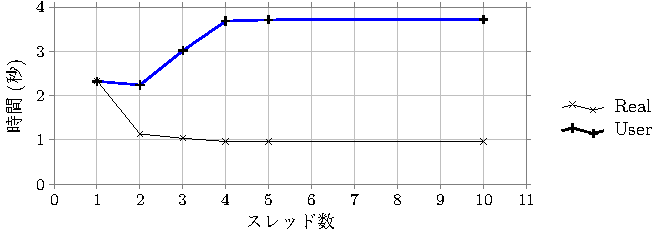
\includegraphics[scale=1.0]{Tbl/threadTimeGrph.pdf}
\end{myfig}

スレッド数が1の時は,経過時間(Real)とユーザCPU時間(User)が,
ほぼ,同じになる.
一つのコア\footnote{従来のCPUのこと.}が全力で合計を計算した結果である.

スレッド数が1〜6の間は,経過時間がスレッド数に反比例して短くなる.
合計の計算時間に対応するユーザCPU時間は,ほぼ一定である.
使用したコンピュータが持つ六つのコアが,
最大で六つのスレッドに割当てられ,
真に並列実行された結果である.

スレッドの数が6〜10に増加する間,経過時間は,ほぼ一定である.
しかしユーザCPU時間が増加している.
必要な計算量は一定なのに長いCPU時間を必要とするので,
コアの性能が悪化したように見える.

コアの性能が悪くなったように見えるのは,
ハイパースレッディング・テクノロジー\cite{hyperThreading}により,
コアの数が倍(12個)あるように見せかけているためである.
ハイパースレッディング・テクノロジーは,
単一スレッドを実行する場合は遊んでしまうコア内のユニットを,
二つのスレッドを同時に実行することで効率よく使用する技術である.
見かけ上コアの数が二倍になるが,合計の性能は二倍には達しないので,
コアあたりの性能が下がったように見える.
%\footnote{
%この計測結果からは,
%ハイパースレッディング・テクノロジーは,
%性能の改善に余り寄与していないように見える.
%}

%スレッド数を12以上にすると,
%(見かけ上の)コア全てが常時使用されるので,
%経過時間,ユーザ時間の合計のどちらも一定になる.

%==============================================================================
\section{CPU仮想化の実装例}
第\ref{tacosVirtualCPU}章にTacOSのCPU仮想化の例を示す.
この例は,{\cmml}で記述したカーネル内データ構造や,
プロセス切換えプログラム,プロセススケジューラ等の実装を含む.
また,プロセスのメモリ配置についても説明している.

%==============================================================================
\section{まとめ}
本章では,時分割多重によるCPUの仮想化について学んだ.
プロセスは幾つかの状態を持ち,
実行できない状態の場合はCPUを割当てない.
プロセスはイベントやタイムスライシングにより状態が変化する.
CPUは,実行を中断するプロセスから次に実行するプロセスに,
コンテキストスイッチを行う.

PCBはプロセスを表現するカーネル内の重要なデータ構造である.
例えばプロセスの待ち行列はPCBの待ち行列として表現されるし,
プロセスの実行が中断する時はPCBにコンテキストが保存される.

スレッドを導入することで,
SMPに対応したプロセスのモデルを表現できる.
スレッドにはカーネルスレッドとユーザスレッドがあった.
また,これらを組み合わせた三つのスレッドモデルがあった.
POSIXスレッドを用いてデータの合計を計算する処理を高速化する
プログラム例を紹介し,実行時間の計測結果を示した.
スレッド数がCPU(コア)数以内の場合は,
スレッド数に反比例して実行時間が短くなることが確認できた.

%==============================================================================
\section*{練習問題}
\begin{enumerate}
  \renewcommand{\labelenumi}{\ttfamily\arabic{chapter}.\arabic{enumi}}
  \setlength{\leftskip}{1em}
\item 次の言葉の意味を説明しなさい.
  \begin{enumerate}
    \item 時分割多重
    \item コンテキストスイッチ
    \item Dispatch(ディスパッチ)
    \item Preemption(プリエンプション)
    \item プロセスの状態
    \item プロセスの状態遷移
    \item RETI命令
    \item PCB
    \item 待ち行列
    \item 実行可能列
    \item スレッド
    \item カーネルスレッド
    \item ユーザスレッド
    \item One-to-One Model
    \item Many-to-One Model
    \item Many-to-Many Model
  \end{enumerate}
\item POSIXスレッドについて調査しなさい.
\end{enumerate}
 % CPUの仮想化

\begin{thebibliography}{9}

\bibitem{tec}
重村哲至,古川達也,相知政司,林 敏浩:
コンソールパネルを持つ機械語教育用マイコンの開発と授業への応用,
情報処理学会論文誌,Vol.48,No.9,pp.3318--3327(2007).

\bibitem{os360}
ウキペディア,
OS/360,
\url{https://ja.wikipedia.org/wiki/OS/360}(2017.10.03 閲覧)

\bibitem{mvs}
ウキペディア,
MVS,
\url{https://ja.wikipedia.org/wiki/Multiple_Virtual_Storage}(2017.10.03 閲覧)

\bibitem{os390}
ウキペディア,
OS/390,
\url{https://ja.wikipedia.org/wiki/OS/390}(2017.10.03 閲覧)

\bibitem{zos}
ウキペディア,
z/OS,
\url{https://ja.wikipedia.org/wiki/Z/OS}(2017.10.03 閲覧)

\bibitem{unix}
ウキペディア,
UNIX(「UNIXおよびUNIX系システムの系統図」を含む),
\url{https://ja.wikipedia.org/wiki/UNIX}(2017.10.03 閲覧)

\bibitem{solaris}
ウキペディア,
Solaris,
\url{https://ja.wikipedia.org/wiki/Solaris}(2017.10.03 閲覧)

\bibitem{aix}
ウキペディア,
AIX,
\url{https://ja.wikipedia.org/wiki/AIX}(2017.10.03 閲覧)

\bibitem{mach}
ウキペディア,
Mach,
\url{https://ja.wikipedia.org/wiki/Mach}(2017.10.03 閲覧)

\bibitem{bsdd}
ウキペディア,
BSDの子孫,
\url{https://ja.wikipedia.org/wiki/BSD%E3%81%AE%E5%AD%90%E5%AD%AB}(2017.10.03 閲覧)

\bibitem{bsd}
ウキペディア,
BSD,
\url{https://ja.wikipedia.org/wiki/BSD}(2017.10.04 閲覧)

\bibitem{386bsd}
ウキペディア,
386BSD,
\url{https://ja.wikipedia.org/wiki/386BSD}(2017.10.04 閲覧)

\bibitem{freebsd}
ウキペディア,
FreeBSD,
\url{https://ja.wikipedia.org/wiki/FreeBSD}(2017.10.03 閲覧)

\bibitem{freenas}
ウキペディア,
FreeNAS,
\url{https://ja.wikipedia.org/wiki/FreeNAS}(2017.10.03 閲覧)

\bibitem{nextstep}
ウキペディア,
NEXTSTEP,
\url{https://ja.wikipedia.org/wiki/NEXTSTEP}(2017.10.03 閲覧)

\bibitem{classicmacos}
ウキペディア,
Classic Mac OS,
\url{https://ja.wikipedia.org/wiki/Classic_Mac_OS}(2017.10.03 閲覧)

\bibitem{dynabook}
ウキペディア,
ダイナブック,
\url{
https://ja.wikipedia.org/wiki/ダイナブック
}(2017.10.03 閲覧)

\bibitem{macos}
ウキペディア,
macOS,
\url{
https://ja.wikipedia.org/wiki/MacOS
}(2017.10.03 閲覧)

\bibitem{ios}
ウキペディア,
iOS (アップル),
\url{
https://ja.wikipedia.org/wiki/IOS_(アップル)
}(2017.10.03 閲覧)

\bibitem{linux}
ウキペディア,
Linux,
\url{
https://ja.wikipedia.org/wiki/Linux
}(2017.10.03 閲覧)

\bibitem{android}
ウキペディア,
Andriod,
\url{
https://ja.wikipedia.org/wiki/Android
}(2017.10.03 閲覧)

\bibitem{msdos}
ウキペディア,
MS-DOS,
\url{
https://ja.wikipedia.org/wiki/MS-DOS
}(2017.10.03 閲覧)

\bibitem{windows}
ウキペディア,
Microsoft Windows(「Windows ファミリー系統図」含む),
\url{
https://ja.wikipedia.org/wiki/Microsoft_Windows
}(2017.10.03 閲覧)

\bibitem{ibmpc81}
ウキペディア,IBM PC,
\url{
https://ja.wikipedia.org/wiki/IBM_PC
}(2017.10.04 閲覧)

\bibitem{svr4}
ウキペディア,UNIX System V,
\url{
https://ja.wikipedia.org/wiki/UNIX_System_V
}(2017.10.04 閲覧)

\bibitem{iebsd}
重村哲至,情報電子工学科電算機室におけるPC-UNIXの歴史,
\url{
http://www2.tokuyama.ac.jp/giga/Sigemura/Public/IeNet/history.html
}(2017.10.03 閲覧)

\bibitem{linux1}
Linux kernel release 1.0,
\url{
https://www.kernel.org/pub/linux/kernel/v1.0/linux-1.0.tar.gz
}(2017.10.04)

\bibitem{third}
Andrew S. Tanenbaum, Herbert Bos:
``The Third Generaton(1965--1980):ICs and Multiproguramming'',
Modern Operating Systems(4th Edition),pp.9-14,
Pearson Education,Inc(2014).

\bibitem{fourth}
Andrew S. Tanenbaum, Herbert Bos:
``The Fourth Generation(1980--Present):Personal Computers'',
Modern Operating Systems(4th Edition),pp.15--19,
Pearson Education,Inc(2014).

\bibitem{key72}
Alan C. Kay:
``A Personal Computer for Children of All Ages'',
Proceeding ACM '72 Proceedings of the ACM annual conference - Volume 1
Article No 1 (1972).

\bibitem{key72J}
アラン・ケイ:すべての年齢の「子供たち」のためのパーソナルコンピュータ,
阿部和広,小学生からはじめるわくわくプログラミング,pp.130--141,
日経BP社(2013).

\bibitem{dynabook2}
アラン・ケイ:Dynabookとは何か?
「すべての年齢の「子供たち」のためのパーソナルコンピュータ」の後日談,
阿部和広,小学生からはじめるわくわくプログラミング,pp.142--149,
日経BP社(2013).

\bibitem{kei}
師尾 潤 他:スーパーコンピュータ「京」のオペレーティングシステム,
\url{http://img.jp.fujitsu.com/downloads/jp/jmag/vol63-3/paper07.pdf}
(2017.10.03 閲覧),
富士通(2012).

\bibitem{zfs}
Marshall Kirk McKusick,
George V. Neville-Neil,
Robert N. M. Watson:``The Zettabyte Filesystem,''
The Design and Implementation of the FreeBSD Operating System
Second Edition,Pearson Education,Inc,pp.523-550(2015).

%\bibitem{cpmJ}
%アンドリュー・S・タネンバウム,
%モダンオペレーティングシステム原著第2版,13ページ,
%ピアソン・エデュケーション(2004).

\bibitem{lines}
Andrew S. Tanenbaum, Herbert Bos:
``INTRODUCTION'',
Modern Operating Systems(4th Edition),pp.1-3,
Pearson Education,Inc(2014).

\bibitem{virtualization}
Andrew S. Tanenbaum, Herbert Bos:
``VIRTUALIZATION AND THE CLOUD'',
Modern Operating Systems(4th Edition),pp.471-516,
Pearson Education,Inc(2014).

\bibitem{vsphere}
ヴイエムウェア株式会社:
``VMware 徹底入門 第3版'',
廣済堂(2012).

\bibitem{ubuntu}
仮想ハードディスクイメージのダウンロード,
\url{https://www.ubuntulinux.jp/download/ja-remix-vhd}
(2017.10.19 閲覧),
Ubuntu Japanese Team(2012).

\bibitem{lightWeight}
Andrew S. Tanenbaum, Herbert Bos:
``Thread Usage'',
Modern Operating Systems(4th Edition),pp.97-102,
Pearson Education,Inc(2014).

\bibitem{hyperThreading}
ウキペディア,ハイパースレッディング・テクノロジー,
\url{
https://ja.wikipedia.org/wiki/%E3%83%8F%E3%82%A4%E3%83%91%E3%83%BC%E3%82%B9%E3%83%AC%E3%83%83%E3%83%87%E3%82%A3%E3%83%B3%E3%82%B0%E3%83%BB%E3%83%86%E3%82%AF%E3%83%8E%E3%83%AD%E3%82%B8%E3%83%BC
}(2017.11.02 閲覧)

\bibitem{AbstractDataType}
B.H.Liskov, S.N.Zilles:``Programming with Abstract Data Type'',
SIGPLAN Notices,9,4,pp.50-59(1974).

\bibitem{MemoryAllocation}
Abraham Silberschatz, Peter Baer Galvin, Greg Gagne:
``Memory Allocation'',
Operating System Concepts(9th Edition), pp.362-363,
John Wiley \& Sons,Inc(2013).

\bibitem{ia32Segmentation}
John H. Crawford, Patrick P. Gelsinger:``ベースとリミット'',
80386プログラミング, 工学社, pp.413-414(1988).

\bibitem{ia32SegmentReg}
John H. Crawford, Patrick P. Gelsinger:
``セグメント部:セグメント・レジスタ'',
80386プログラミング, 工学社, pp.48-50(1988).

\bibitem{ia32SegmentHiddenReg}
John H. Crawford, Patrick P. Gelsinger:
``デスクリプタ用の裏レジスタ'',
80386プログラミング, 工学社, pp.420-421(1988).

\bibitem{invertedPageTable}
Albert Chang, Mark F. Mergen:
``801 storage: architecture and programming'',
ACM Transactions on Computer Systems, 6, 1,
pp.28-50 (1988).

\bibitem{execOfFreeBSD}
Marshall Kirk McKusick,
George V. Neville-Neil,
Robert N. M. Watson:``Execution of a File'',
The Design and Implementation of the FreeBSD Operating System
Second Edition,Pearson Education,Inc,pp.262-263(2015).

\bibitem{wsClock}
Andrew S. Tanenbaum, Herbert Bos:
``The WSClock Page Replacement Algorithm'',
Modern Operating Systems(4th Edition),pp.219-221,
Pearson Education,Inc(2014).

\bibitem{RaidzOfFreeBSD}
Marshall Kirk McKusick,
George V. Neville-Neil,
Robert N. M. Watson:``RAIDZ'',
The Design and Implementation of the FreeBSD Operating System
Second Edition,Pearson Education,Inc,pp.540-541(2015).

\bibitem{DeduplicationOfFreeBSD}
Marshall Kirk McKusick,
George V. Neville-Neil,
Robert N. M. Watson:``Dedupliation'',
The Design and Implementation of the FreeBSD Operating System
Second Edition,Pearson Education,Inc,pp.545-546(2015).

\end{thebibliography}
 % 参考文献

%\appendix
%\chapter{TaCに関する資料}
\label{appTac}

%==============================================================================
\section{CPUの概要}
TaCで使用できるデータの形式,
CPU内部のレジスタ構成,
機械語命令について説明する.

\subsection{データ形式}
\figref{tacData}にTaCが扱うことができるデータ形式を示す.
16ビットの整数データと,16ビットのアドレスデータの他に,
8ビットのデータを扱うことができる.
16ビットのデータはCPUの内部でもメモリやI/Oでも使用できる.
メモリやI/Oの16ビットデータにアクセスする場合は偶数番地を用いる.
8ビットデータはメモリとI/Oの読み書きだけに使用できる.
メモリやI/Oの8ビットデータにアクセスする場合は,
CPUレジスタの下位8ビットが使用される.

\begin{myfig}{btp}{データ形式}{tacData}
  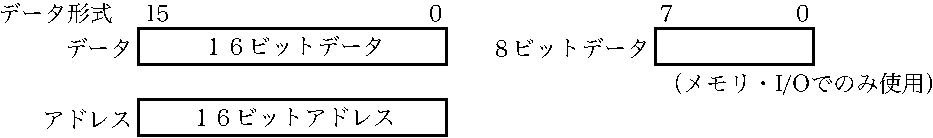
\includegraphics[scale=0.7]{Tbl/TaC7a-instruction-p1-1-crop.pdf}
\end{myfig}

\subsection{CPUレジスタとPSW}
\figref{tacRegPsw}にCPU内部のレジスタなどを示す.
レジスタはどれも16ビット幅である.
CPUレジスタは,
汎用のG0からG11,
フレームポインタとして使用するFP,
カーネルモード用のスタックポインタSSP,
ユーザモード用のスタックポインタUSPからなる.
これらは全て計算用にもアドレス用にも使用できる.
FP,SSP,USPは,以下に説明する特別な意味も持っている.

FPはフレームポインタ相対アドレッシングモードで使用できる.
このアドレッシングモードを用いると,
スタックフレーム内のローカル変数や関数引数へ,
1ワードの機械語命令でアクセスできる.

SSPはカーネルモードでSPの位置にマップされスタックポインタとして使用される.
USPはユーザモードでSPの位置にマップされスタックポインタとして使用される.
USPは最後のレジスタとして常時マップされており,
カーネルモードでもUSPをアクセスすることができる.

PSWはPCとFLAGからなる.
PCはプログラムカウンタのことである.
FLAGには,計算結果で変化するV,C,S,Zと,
割込み許可E,カーネルモードPの各ビットがある.
割込みが発生するとPCとFLAGが順にカーネルスタックにPUSHされた後で,
割込みが禁止された上でカーネルモードに切り換わる
(Eビットが0,Pビットが1になる).

\begin{myfig}{btp}{CPU内部の記憶装置}{tacRegPsw}
  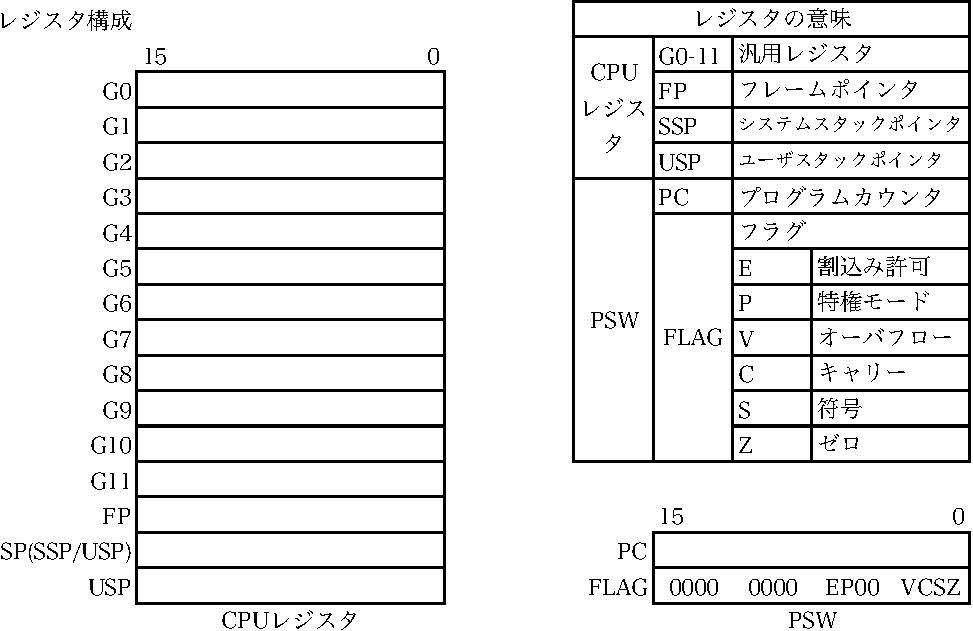
\includegraphics[scale=0.7]{Tbl/TaC7a-instruction-p1-3-crop.pdf}
\end{myfig}

\subsection{機械語命令}
\figref{tacInsTbl}にTaCの機械語命令の一覧表を示す.
IN,OUT,RETI,EI,DI,HALTはカーネルモードでしか使用できない特権命令である.
SVC命令はシステムコールを発行するためにSVC割込みを発生する.

ほとんどの転送命令と計算命令で8種類のアドレッシング・モードが使用できる.
Direct,Indexed,Immediateの
三つのアドレッシング・モードを使用する場合は2ワードの機械語命令になる.
他のアドレッシング・モードの場合は全て1ワード命令である.

Byte Register Indirect アドレッシング・モードだけが,
メモリの8ビットデータをアクセスする.
Byte Register Indirect アドレッシング・モードの
ST命令はCPUレジスタの下位8ビットがメモリに書き込まれる.
その他の命令ではメモリから読み出した8ビットデータの上位に
\|00h|を付加した16ビットデータに変換して使用する.

\begin{myfig}{btp}{命令表}{tacInsTbl}
  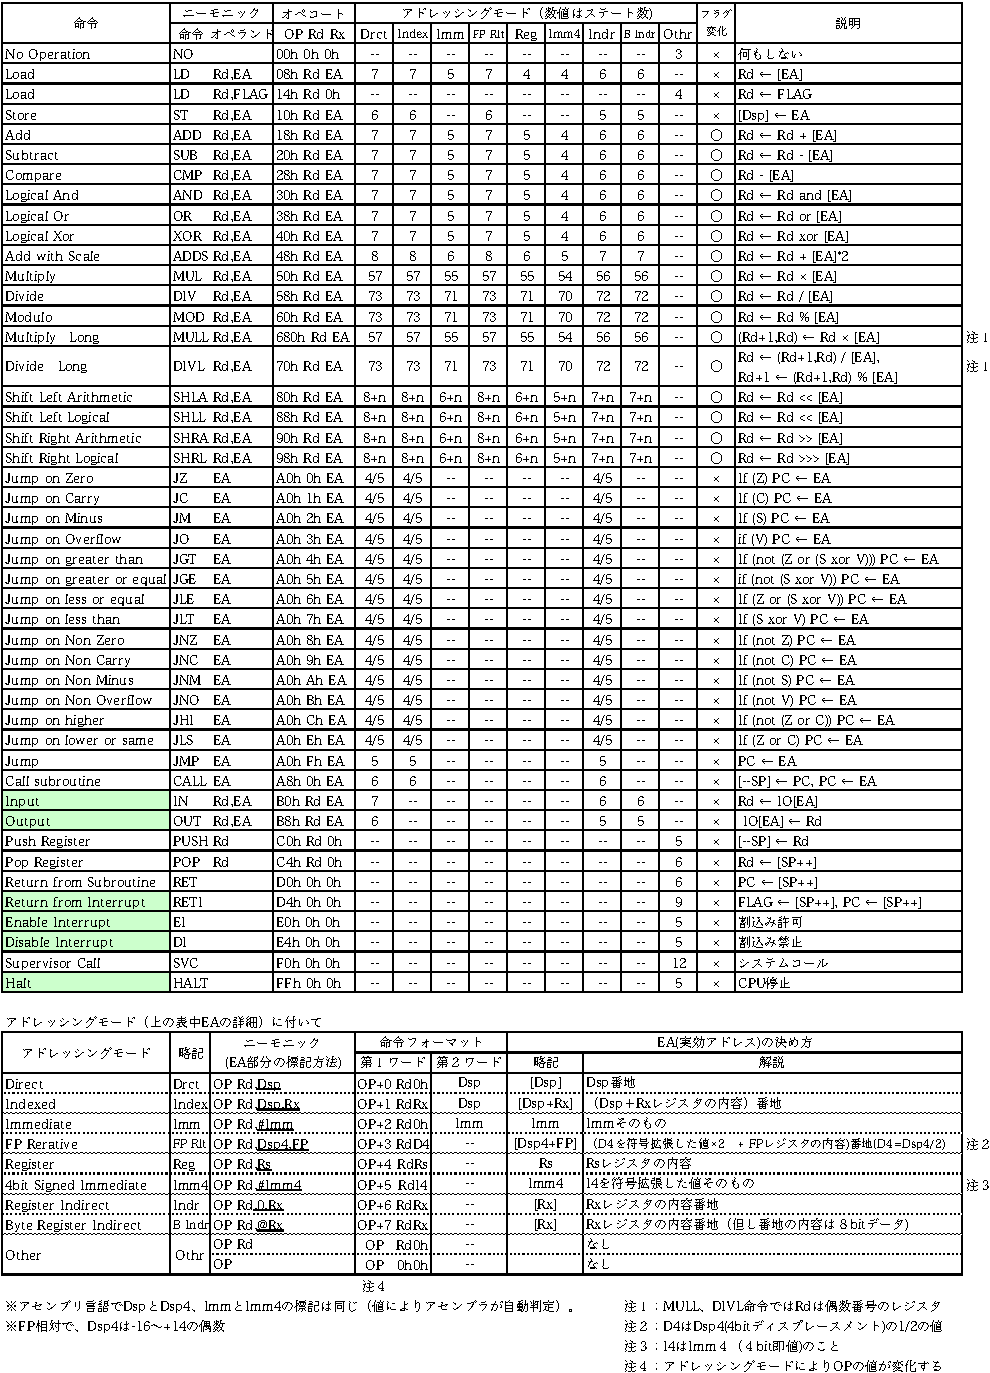
\includegraphics[scale=0.94]{Tbl/TaC7a-instruction-p2-crop.pdf}
\end{myfig}

%==============================================================================
\newpage
\section{メモリマップとI/Oマップ}
\figref{tacMap}にTaCのメモリマップとI/Oマップを示す.
メモリやI/Oは8ビット毎にアドレス付けされており,
8ビットデータ,16ビットデータのどちらも読み書きできる.
アドレッシング・モードによって,8ビットデータと16ビットデータの区別をする.
16ビットデータは偶数アドレスを指定してアクセスしなければならない.

\subsection{メモリ空間}
TaCのメモリ空間は\|0000h|から\|FFFFh|の64KiBである.
16ビットデータは偶数アドレスからの2バイトに配置され,
偶数アドレスを指定してアクセスする.
16ビットデータにアクセスするには,
Byte Register Indirect モード\emph{以外}のアドレッシング・モードを用いる.
8ビットデータにアクセスするには,
Byte Register Indirect モードを用いる.

メモリ空間の最初から56KiBは自由に使用できるメモリであり,
ここにTacOSのカーネルやユーザプロセスがロードされる.
\|E000h|から\|EFFFh|まではVRAMが配置されている.
VRAMにASCIIコードを書き込むと対応する文字がディスプレイに表示される.
VRAMのアドレスがディスプレイの表示位置に対応する.
\|F000h|から\|FFDFh|はIPL(ROM)が配置される.
IPLはマイクロSDカードからTacOSを読み出して起動する.
\|FFE0h|から\|FFFFh|は割込みベクタ領域である.
16種類の割込みに対応するハンドラの入口番地をTacOSがセットする.

\subsection{I/O空間}
TaCのI/O空間は\|00h|から\|FFh|の256Bである.
I/O空間のアドレス幅は8ビットだが,
IN,OUT命令ではI/Oアドレスが16ビットで表現される.
I/Oアドレスの上位8ビットは\|00h|になるようにする.
上位8ビットが\|00h|以外になった場合の動作は保証されない.

メモリ空間と同様に8ビットデータと16ビットデータの両方を読み書きできる.
8ビットデータと16ビットデータの区別は,
IN,OUT命令のアドレッシングモードにより行う.
I/Oの8ビットデータにアクセスするには,
Byte Register Indirect モードを用いる.

\begin{myfig}{btp}{メモリマップとI/Oマップ}{tacMap}
  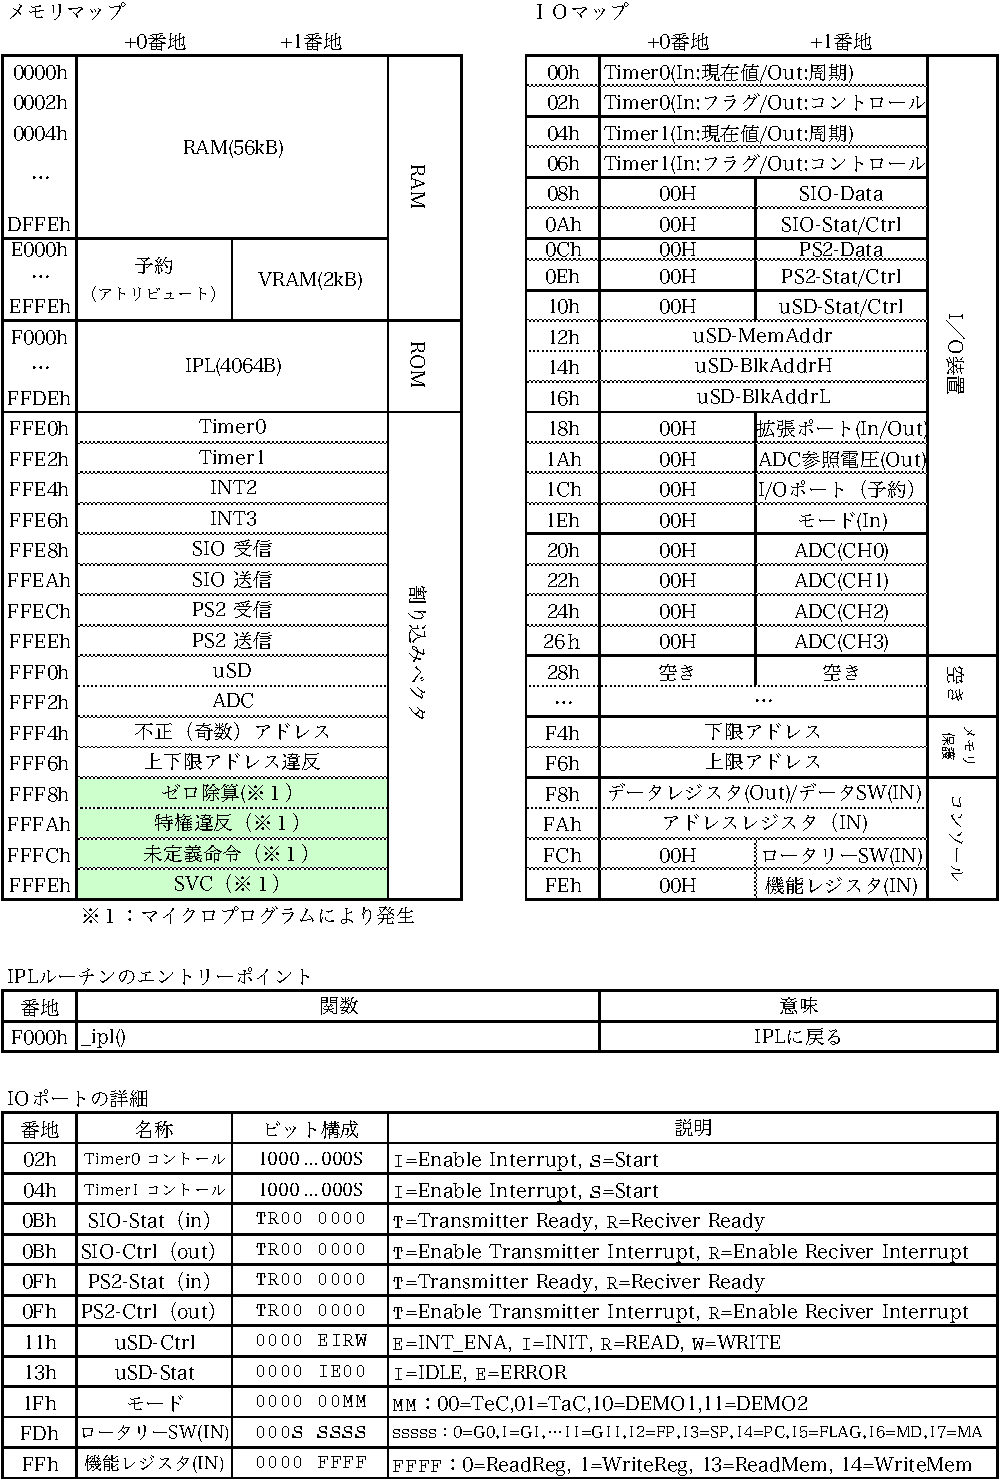
\includegraphics[scale=0.8]{Tbl/TaC7a-instruction-p4-crop.pdf}
\end{myfig}
  % 付録A

%------------------------------------------------------------------------------
% 発行元
\backmatter
\pagestyle{empty}
\onecolumn
~
\vfill\vfill\vfill
\begin{center}
\fbox{\parbox{10cm}{ \vspace{0.3cm}
\large{\bf{オペレーティングシステム Ver. 0.0.0}} \\
\\
 発行年月 2017年10月 Ver.0.0.0 \\
 発  行 独立行政法人国立高等専門学校機構 \\
      徳山工業高等専門学校 \\
      情報電子工学科 重村哲至 \\
      〒745-8585 山口県周南市学園台 \\
      sigemura@tokuyama.ac.jp \\
}}
\end{center}
\vfill
\end{document}
